% Complete source. Build with pdflatex twice. No shell escape or external figures.
\documentclass[11pt]{article}
\pdfinfoomitdate=1
\pdftrailerid{}
\pdfsuppressptexinfo=15
\usepackage[a4paper,margin=22mm,headheight=14pt,headsep=7mm,footskip=11mm]{geometry}
\usepackage[T1]{fontenc}
\usepackage[utf8]{inputenc}
\usepackage{lmodern,microtype,amsmath,amssymb,amsthm,graphicx,booktabs,tabularx,longtable,array}
\usepackage{tikz,pgfplots,tcolorbox,enumitem,fancyhdr,titlesec,caption,placeins,xurl}
\usepackage[numbers,sort&compress]{natbib}
\usepackage[colorlinks=true,linkcolor=Cosmic,citecolor=Cosmic,urlcolor=Cosmic,breaklinks=true]{hyperref}
\usetikzlibrary{arrows.meta,positioning,calc,fit,backgrounds,shapes.geometric}
\pgfplotsset{compat=1.18}
\definecolor{Cosmic}{HTML}{40205E}
\definecolor{Violet}{HTML}{7544B8}
\definecolor{Lilac}{HTML}{C4AAEC}
\definecolor{Mist}{HTML}{F3EFF8}
\definecolor{Ink}{HTML}{211C2B}
\definecolor{Muted}{HTML}{655D72}
\definecolor{Teal}{HTML}{146D63}
\definecolor{Mint}{HTML}{EAF6F1}
\definecolor{Amber}{HTML}{935815}
\definecolor{Sand}{HTML}{FFF5E7}
\definecolor{Rose}{HTML}{A5395B}
\color{Ink}
\setlength{\parindent}{0pt}
\setlength{\parskip}{5.5pt plus 1pt minus 1pt}
\setlength{\emergencystretch}{2em}
\setlength{\tabcolsep}{4.5pt}
\renewcommand{\arraystretch}{1.18}
\setlist[itemize]{leftmargin=1.3em,topsep=3pt,itemsep=2pt}
\setlist[enumerate]{leftmargin=1.6em,topsep=3pt,itemsep=2pt}
\titleformat{\section}{\Large\sffamily\bfseries\color{Cosmic}}{\thesection}{.65em}{}
\titleformat{\subsection}{\large\sffamily\bfseries\color{Cosmic}}{\thesubsection}{.65em}{}
\titleformat{\subsubsection}{\normalsize\sffamily\bfseries\color{Cosmic}}{\thesubsubsection}{.65em}{}
\titlespacing*{\section}{0pt}{18pt}{8pt}
\titlespacing*{\subsection}{0pt}{12pt}{4pt}
\captionsetup{font=small,labelfont={bf,color=Cosmic},justification=raggedright,singlelinecheck=false}
\pagestyle{fancy}\fancyhf{}
\fancyhead[L]{\scriptsize\sffamily\color{Cosmic}SUCCESSOR $\Omega$ HARNESS}
\fancyhead[R]{\scriptsize\sffamily\color{Muted}MAKE EVERY MISSION BUILD WHAT COMES NEXT}
\fancyfoot[L]{\scriptsize\sffamily\color{Muted}MONTREAL.AI\quad Research edition 01\quad 24 October 2026}
\fancyfoot[R]{\small\sffamily\color{Cosmic}\thepage}
\renewcommand{\headrulewidth}{.3pt}
\newtcolorbox{insight}[1][]{colback=Mist,colframe=Lilac,boxrule=.5pt,arc=2pt,left=9pt,right=9pt,top=7pt,bottom=7pt,fonttitle=\sffamily\bfseries,coltitle=Cosmic,#1}
\newtcolorbox{boundary}[1][]{colback=Sand,colframe=Amber!35,boxrule=.5pt,arc=2pt,left=9pt,right=9pt,top=7pt,bottom=7pt,fonttitle=\sffamily\bfseries,coltitle=Amber,#1}
\newcolumntype{Y}{>{\raggedright\arraybackslash}X}
\newcolumntype{P}[1]{>{\raggedright\arraybackslash}p{#1}}
\newtheorem{proposition}{Proposition}
\newtheorem{definition}{Definition}
\newcommand{\Harness}{SUCCESSOR $\Omega$ Harness}
\newcommand{\TI}{TRANSFORMATIONAL INTELLIGENCE $\infty$}
\newcommand{\code}[1]{\texttt{#1}}
\newcommand{\status}[1]{\textsf{\textbf{#1}}}
\hypersetup{pdftitle={SUCCESSOR Omega Harness: Make Every Mission Build What Comes Next},pdfauthor={MONTREAL.AI},pdfsubject={Scientific capability construction, provenance, fresh qualification and bounded successor execution},pdfkeywords={SUCCESSOR Omega, Transformational Intelligence, capability inheritance, instrumentation, reproducibility, durable workflows}}
\begin{document}
\hypersetup{pageanchor=false}

% BEGIN sections/cover.tex
\begin{titlepage}
\thispagestyle{empty}

\begin{tikzpicture}[remember picture,overlay]
\fill[Cosmic!64!black] (current page.south west) rectangle (current page.north east);
\begin{scope}[shift={(current page.south west)},x=1cm,y=1cm]
\foreach \x/\y/\r in {1.1/28/.022,4.4/28.5/.014,8.2/27.8/.018,13/28.3/.015,19.5/27/.020,18/25/.014,20/22/.018,19.7/18/.013,1.3/20/.012,1.4/14/.016,19/13/.016,18.7/9/.014,20/5/.022,17/3/.013,9/1.1/.015,5/1.4/.016,1.5/3/.018,15/26/.012,17/22/.01,19.1/21/.01,14.5/17/.01}
\fill[white,opacity=.5] (\x,\y) circle[radius=\r];
\draw[Lilac,opacity=.18,line width=.7pt] (17.6,24.5) circle[radius=3.25];
\draw[Lilac,opacity=.11,line width=.7pt] (17.6,24.5) circle[radius=3.85];
\node[text=white,opacity=.11,font=\fontsize{120}{120}\selectfont] at (17.6,24.5) {$\Omega$};
\node[anchor=west,text=Lilac,font=\sffamily\small] at (2.2,27.2) {MONTREAL.AI\quad /\quad RESEARCH \& ENGINEERING};
\node[anchor=north west,text=white,text width=16cm,font=\sffamily\bfseries\fontsize{39}{44}\selectfont,align=left] at (2.15,23.4) {SUCCESSOR $\Omega$\\HARNESS};
\node[anchor=north west,text=white,text width=15.7cm,font=\sffamily\fontsize{23}{29}\selectfont,align=left] at (2.2,19.3) {Make Every Mission\\Build What Comes Next};
\draw[Lilac,line width=1pt] (2.2,15.8)--(5.2,15.8);
\node[anchor=north west,text=Lilac,text width=15.7cm,font=\sffamily\fontsize{12}{17}\selectfont,align=left] at (2.2,14.9) {Powered by\\TRANSFORMATIONAL INTELLIGENCE $\infty$.};
\node[anchor=north west,text=white,text width=15.7cm,font=\sffamily\fontsize{12}{17}\selectfont,align=left] at (2.2,12.7) {For TRANSFORMATIONAL AUTONOMOUS ENTERPRISES:\\ACTIVATE. EVOLVE. SCALE.};
\node[anchor=north west,text=white,text width=14.7cm,font=\sffamily\bfseries\fontsize{15}{21}\selectfont,align=left] at (2.2,8.6) {From a completed measurement\\to the means of a new investigation.};
\node[anchor=north west,text=Lilac,text width=15.5cm,font=\sffamily\small,align=left] at (2.2,5.55) {A source-pinned, wallet-free research demonstration.\\Scientific models, exact constructions, fair comparisons,\\and an inspectable boundary between evidence and authority.};
\node[anchor=west,text=Lilac,font=\sffamily\small] at (2.2,2.45) {24 OCTOBER 2026\quad $\cdot$\quad PHOTOMETER EDITION 01};
\end{scope}
\end{tikzpicture}
\null
\end{titlepage}

% END input

\hypersetup{pageanchor=true}
\setcounter{page}{1}

% BEGIN sections/abstract.tex
\begin{center}
{\Large\sffamily\bfseries\color{Cosmic}Make Every Mission Build What Comes Next\par}
\vspace{5pt}
{\small\sffamily MONTREAL.AI\quad Research and engineering edition\par}
\end{center}
\begin{abstract}
A completed mission can leave a useful answer without leaving a usable capability. We investigate a thin execution layer that retains constructed artifacts and provenance while requiring a successor to earn fresh qualification and separately scoped authority. A source-pinned research adapter extends the released AGI ALPHA job dispatcher with an exact-arithmetic virtual photometer: a calibrated scalar instrument becomes a jointly decoded two-signal instrument under a twelve-acquisition cap. The child consumes its parent's constructed nuisance-model recipe, while its decoder, calibration, proof and permission are new. The joint program uses twelve reference-plus-sample readings where two separately calibrated scalar procedures require sixteen; a competent conventional joint construction can match it. A protocol frozen before evaluation compares four methods across four held-out campaigns of 48 missions. All methods qualify all 192 missions per method under the fixed resource vector. Harness scientific reuse and equally capable conventional reuse match exactly at 609,524 counted rational operations and 2,112 simulated detector readings each. Exhaustive rebuilding uses 7,953,264 operations, while a sufficient expert-coded construction wins at 169,732. Inheritance itself is not always cheaper: the first scalar-to-joint transition adds 49 operations relative to fresh direct construction. Released-source runtime experiments retain interruption and recovery history, reject stale proof/permission and expose journal custody assumptions. Two out-of-model controls pass internal validation while giving scientifically wrong answers. The result is an inspectable, conditional capability transition, not a new workflow primitive, physical-instrument validation, complete economic advantage or four-product deployed integration.
\end{abstract}
\noindent\textbf{Keywords:} capability construction; scientific instrumentation; fresh qualification; durable execution; provenance; bounded authority; reproducible research.

\begin{insight}[title={The result to remember}]
The new instrument changes what is feasible. Reuse changes the cost of repeating it.\newline
The harness preserves what happened and what may happen next.\newline
None of these, alone, guarantees truth, superiority or permission.
\end{insight}

\noindent\textbf{Evidence scope.} Exact finite mathematics, actual local scientific computation and released runtime source execution. The detector and role identities are synthetic. Installed four-product execution, physical measurement and financial settlement are not established. The complete source, frozen protocols, raw results, failures and independent replay record accompany this manuscript.

% END input


% BEGIN sections/opening.tex
\section{A mission can leave a better starting point}
\label{sec:opening}

Imagine an instrument that cannot reliably see a faint signal because its background changes during measurement. One mission constructs a calibrated measurement program that cancels that background. The useful output is a measured value. The more durable output is an inspectable way of measuring: a model, an executable estimator, an error bound, a validation procedure, and a record of where each is allowed to apply.

Now ask a different question. Can the same apparatus separate two overlapping signals under the same twelve-reading cap? A saved scalar answer cannot do this. A saved scalar proof cannot certify it. Some machinery remains valuable, but the signal representation and measurement program must change. If the new construction fails, retaining the old instrument or stopping is an acceptable outcome.

This is the concrete meaning of the title's promise. \emph{Make every mission build what comes next} is a design objective that can fail a test. A mission can produce negative evidence, an explicit impossibility result, or a decision to stop rather than a valuable descendant. We investigate conditions under which completed work preserves and transforms the means of doing subsequent useful work, while charging for the transformation and respecting its limits.

\begin{insight}[title={The research question}]
Under what conditions can a lightweight harness turn completed work into transferable productive capability, while preserving evidence, controlling authority, and reducing the total cost of subsequent qualified missions?
\end{insight}

The paper answers this question at three levels. Mathematically, a finite measurement model makes the change in feasibility explicit. Operationally, actual callbacks run through the released AGI ALPHA job dispatcher, with durable records, source-bound work receipts, validation and recovery. Empirically, a frozen synthetic study gives competent conventional reuse and a supplied expert construction the same tools, cached artifacts, validators and resource constraints. These levels support different claims. A rank calculation is not physical instrument validation; a valid local journal is not independent organizational review; an existing product release is not qualification of a new connected deployment.

\subsection{The three-minute experience}

The companion opens with a virtual photometer and one question: \emph{What remains of the signal after the background is removed?} The reader runs the actual local mission, examines the measurement weights and retained evidence, then requests the two-signal successor. The display separates the acquired readings from the estimated signals and shows what the successor must construct afresh. The reader can inspect a detected invalid proposal, an out-of-model failure, and recovery evidence. Every visible stage links to its actual computation or evidence record; animation is presentation, not execution evidence.

The default experience is local and wallet-free. No chain connection, model-provider credential or remote worker is required. The browser is an interface to a bounded research companion, not a replacement project runtime or a claim that the held production Harness is released. The exact launch commands and evidence levels appear in Section~\ref{sec:reproduction}.

\subsection{What this edition contributes}

The contribution is a reproducible \emph{capability-transition experiment}: a scalar drift-cancelling estimator becomes a two-channel estimator, and the study identifies which structure transfers and which obligations restart. The research adapter binds those computations to an existing execution boundary rather than introducing a second workflow engine. A vector cost ledger keeps acquisition, computation, qualification, recovery and unknown human labor separate. An explicit failure map records both refusals and the scientific failures a structurally correct harness cannot detect.

The paper does not claim to invent durable workflows, event sourcing, linear estimation, access control, caching or capability provenance. Nor does it establish superiority over all competent workflows. Its proposed research contribution is the measured connection between a changed productive constraint, a bounded reusable artifact, and a successor whose evidence and authority are re-established at the point of use.

\subsection{Continuity with prior research}

The project already includes Transformational Intelligence, six Out-stage papers, and earlier autonomous-enterprise and Harness studies \cite{ti,outlearn,outthink,outdesign,outstrategise,outexecute,outevolve,priorharness}. This edition preserves their original artifacts separately. In particular, the earlier work's comparator wins and qualification costs motivate a stronger experiment; they are not replaced by the present results. The prior Harness studies include graph-semantic lowering and other scientific constructions. This paper's distinct empirical object is the transition from one calibrated optical amplitude to a jointly identifiable pair under an acquisition cap.

The project phrase \TI{} names the research discipline used here. It is not an empirical certificate of general intelligence, an unbounded optimization guarantee, or a reason to relax a comparator. The successor earns only the claims supported by its exact world model, policy, evidence and current authorization.

% END input


% BEGIN sections/method.tex
\section{Transformational Intelligence as an executable method}
\label{sec:method}

The foundational TI paper distinguishes searching within a formulation from changing a removable restriction in that formulation. Its causal discipline includes an explicit purpose bridge, an unrestricted same-tools alternative, structural ablations and the possibility of retaining the incumbent \cite{ti}. We apply that discipline to a removable restriction: executing independent scalar measurements when a joint measurement representation can resolve both target signals within a shared acquisition window. The new representation must still satisfy the actual scientific purpose, not merely a convenient internal metric.

\subsection{The source corpus and its limits}

We read the public seven-paper corpus at the frozen Alpha source identified in Section~\ref{sec:system}. The included source manifest records each original PDF and TeX hash. \emph{Out-Learn} constructs informative measurements and calibrates a gain that nuisance cancellation alone cannot remove; its revised drift-cancelling instrument explicitly admits that a conventional specialist can match it \cite{outlearn}. \emph{Out-Think} asks whether a representation preserves the future interface that matters, rather than only today's answer \cite{outthink}. \emph{Out-Design} ties equivalent realizations to useful released capacity, whose location and availability matter \cite{outdesign}. \emph{Out-Strategise} treats information acquisition and construction jointly; uncertainty need not be resolved when one completion works for every surviving case \cite{outstrategise}. \emph{Out-Execute} retains reusable completion boundaries and demands new acceptance when the current witness changes \cite{outexecute}. \emph{Out-Evolve} asks what means of discovery and production can themselves be constructed and inherited \cite{outevolve}.

Those papers use different finite models. Their theorems do not transfer to the photometer merely because a stage has the same name. Their contribution here is a disciplined question for each computation, followed by a new model, new exact checks and new empirical evidence.

\subsection{Seven stages, seven computational obligations}

The seven-stage journey is a semantic view of the research work. It is distinct from the released runtime's seven lifecycle families: constitution, evidence, formation, challenge, verification, admission and renewal. A runtime family constrains who may form, challenge or accept a job; it does not automatically implement learning or design. The adapter records both labels explicitly.

\begin{table}[htbp]
\centering\small
\begin{tabularx}{\linewidth}{P{.15\linewidth}Y Y}
\toprule
\textbf{Stage} & \textbf{Computation and output} & \textbf{Falsifiable contribution}\\
\midrule
Identify & Encode target amplitudes, drift class, error tolerance and acquisition cap; assess the incumbent. & A proposed change must relieve an actual feasibility constraint.\\
Out-Learn & Construct the nuisance representation and calibration specification; execution later obtains the reference readings. & Wrong drift class or gain model invalidates the claimed bound.\\
Out-Think & Compute nuisance rank, necessary observation dimension and decoder obligations; design checks each full candidate. & Collinear signal channels must be rejected as unidentifiable.\\
Out-Design & Solve and compare exact measurement programs with an explicit noise-amplification bound. & Weights must cancel every declared nuisance basis vector and recover every target channel.\\
Out-Strategise & Compute the proposed acquisition cost, compare with the separate-scalar plan, and admit or stop. & A mathematically valid program that exceeds the mission budget is inadmissible.\\
Out-Execute & Acquire simulated reference/sample readings, compute estimates and run fresh independent checks. & Accepted estimates must meet the declared quality threshold on the evaluation bank.\\
Out-Evolve & Package dependencies, applicability, source and evidence; propose a distinct successor. & A child must not inherit a parent's current proof or authority.\\
\bottomrule
\end{tabularx}
\caption{Stage names are useful only when attached to computations, artifacts and possible failure. The companion records stage-specific construction and validation work separately from simulated acquisitions.}
\label{tab:stages}
\end{table}

The method permits early stopping. If the rank test fails, more execution of the same observation scheme cannot fix identifiability. If the quality bound fails, a cheaper but inaccurate program is not useful capacity. If the incumbent is cheaper under the mission's actual constraints, the correct strategy can be retention. These decisions are observable outputs, not exceptions erased from the study.

\subsection{The purpose bridge}

The scientific purpose is recovery of the declared sample amplitudes within an absolute error tolerance using no more than a fixed number of detector acquisitions. The internal algebraic objectives are nuisance annihilation, signal normalization and limited noise amplification. The bridge between them is an explicit error bound and a fresh comparison with simulator ground truth. Cancellation identities alone do not establish purpose: the wrong physical model can satisfy them exactly and still yield the wrong amplitude.

The two-signal request is a real change in the mathematical output contract. Replaying a scalar estimate twice or simply relabelling it does not produce a joint estimator. An expert is free to derive the same joint construction directly. This freedom is necessary to determine whether the benefit arises from the new instrument, from reusable structure, or merely from an artificially weak baseline.

% END input


% BEGIN sections/harness.tex
\section{The minimum harness contract}
\label{sec:harness}

The harness is the thin layer between a mission and attributable bounded execution. It does not decide scientific truth by itself, manufacture demand, or grant a descendant authority by copying its parent's history. In this edition the layer is the existing released Alpha job runtime plus a small application adapter. The scientific constructor remains ordinary pure application code.

\begin{figure}[htbp]
\centering\resizebox{\linewidth}{!}{
% BEGIN figures/architecture.tex
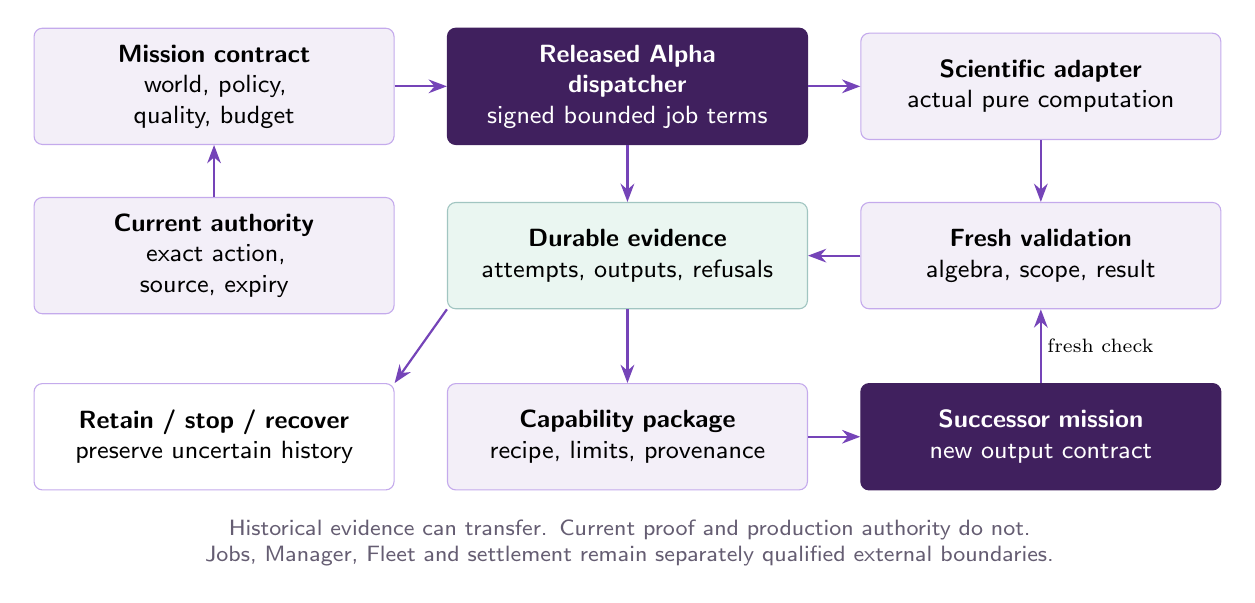
\begin{tikzpicture}[font=\sffamily\small,>=Stealth,
 box/.style={draw=Lilac,fill=Mist,rounded corners=3pt,text width=4.15cm,minimum height=1.35cm,align=center,inner sep=6pt},
 darkbox/.style={box,fill=Cosmic,draw=Cosmic,text=white},
 arr/.style={->,line width=.8pt,draw=Violet}]
\node[box] (mission) at (0,0) {\textbf{Mission contract}\\world, policy,\\quality, budget};
\node[darkbox] (dispatch) at (5.25,0) {\textbf{Released Alpha}\\\textbf{dispatcher}\\signed bounded job terms};
\node[box] (compute) at (10.5,0) {\textbf{Scientific adapter}\\actual pure computation};
\draw[arr] (mission)--(dispatch);
\draw[arr] (dispatch)--(compute);
\node[box] (authority) at (0,-2.15) {\textbf{Current authority}\\exact action,\\source, expiry};
\node[box,fill=Mint,draw=Teal!40] (journal) at (5.25,-2.15) {\textbf{Durable evidence}\\attempts, outputs, refusals};
\node[box] (check) at (10.5,-2.15) {\textbf{Fresh validation}\\algebra, scope, result};
\draw[arr] (authority.north)--(mission.south);
\draw[arr] (dispatch)--(journal);
\draw[arr] (compute)--(check);
\draw[arr] (check)--(journal);
\node[box,fill=white] (stop) at (0,-4.45) {\textbf{Retain / stop / recover}\\preserve uncertain history};
\node[box] (package) at (5.25,-4.45) {\textbf{Capability package}\\recipe, limits, provenance};
\node[darkbox] (child) at (10.5,-4.45) {\textbf{Successor mission}\\new output contract};
\draw[arr] (journal)--(package);
\draw[arr] (journal.south west)--(stop.north east);
\draw[arr] (package)--(child);
\draw[arr] (child.north)--node[right,font=\scriptsize,fill=white,inner sep=2pt]{fresh check}(check.south);
\node[text width=15cm,align=center,font=\sffamily\footnotesize,text=Muted] at (5.25,-5.8) {Historical evidence can transfer. Current proof and production authority do not.\\Jobs, Manager, Fleet and settlement remain separately qualified external boundaries.};
\end{tikzpicture}

% END input
}
\caption{End-to-end architecture of the executed local research path. The application adds scientific callbacks to a released execution boundary. It does not adopt the held Harness overlay or claim current four-product installation.}
\label{fig:architecture}
\end{figure}

\begin{definition}[Mission]
A mission is $M=(\mathcal{W},\mathcal{P},A,B,U,D)$: a declared world model $\mathcal{W}$, policy $\mathcal{P}$, acceptance predicate $A$, resource vector $B$, permitted actions $U$, and a deadline/validity description $D$. A run is qualified only relative to this exact mission and the recorded source and environment.
\end{definition}

The world model names the phenomena and assumptions: polynomial drift, modulation, gain and bounded noise. Policy names what the system is permitted to attempt and what it must refuse. Proof is a scoped statement supported by evidence about a particular implementation and mission. Authority is a current permission to take a particular action. A historical proof can remain historically valid after its permission expires; a current permission does not make a scientific claim true.

\begin{table}[htbp]
\centering\small
\begin{tabularx}{\linewidth}{P{.17\linewidth}Y Y}
\toprule
\textbf{Plane} & \textbf{Concrete example} & \textbf{Transfer rule}\\
\midrule
WORLD & Quadratic background; bounded additive noise; stable gain within a reference/sample pair. & Carry the declared model and evidence; test compatibility with the new requirement.\\
POLICY & Local pure computation; detector-call cap; no remote or financial effects. & Copy as a proposal; the receiving mission must explicitly adopt its policy.\\
PROOF & Exact annihilation identities plus a current fresh error check. & Retain historical evidence with source and scope; new output semantics require new qualification.\\
AUTHORITY & Signed execution authorization bound to job, release, environment and expiry. & Never copy as a production grant. Issue a separately scoped current authorization.\\
\bottomrule
\end{tabularx}
\caption{The four planes are separate even when represented in the same record. A descendant can inherit information without inheriting the right to act.}
\label{tab:planes}
\end{table}

\subsection{Specification, receipts and execution states}

Each job binds immutable terms: mission identity, input/output schema, source release, environment, worker role, acceptance owner, permitted tool, resource reservation, expiry and bounded attempts. The dispatcher seals an acyclic graph, checks input evidence dependencies and prevents a formation worker from owning its challenge, verification or admission. The callback is a locally installed callable; importing arbitrary code is outside this boundary.

The work receipt binds the exact authorization attempt, terms digest, result digest, output types, accepted-by role, validity and permitted uses. The adapter also records the raw scientific artifact hash, not merely a user-facing summary. Receipt validity is distinct from scientific validity: a signed rejected result can be useful work, while a well-formed receipt cannot rescue an invalid estimator.

The lifecycle distinguishes a sealed specification, reserved/dispatched attempt, durable invocation claim, observed completion, accepted or rejected work, and uncertain interruption. Durable STOP, expiry and revocation produce explicit boundary refusals; the released source does not provide a dedicated cancellation-state enumeration or asynchronous preemption. They do not rewrite an earlier accepted record; they change whether that record can currently be used. A new retry receives a new authorization and retains the prior attempt and its resource charge.

\subsection{Durability and uncertain outcomes}

The released journal uses SQLite transactions and hash-linked signed events. The job dispatcher writes an invocation claim before invoking a local handler. Reusing that attempt-scoped invocation identity---institution, job, authorization and invocation identifier---is refused. This closes a common replay path, but it cannot determine an external world's state after every crash. If execution may have happened and completion was not observed, the proper result is uncertainty.

Recovery is a new attributable decision. It identifies the affected job and attempt, preserves the uncertain history and conservatively charges the reserved resources. A later attempt requires fresh authorization. An expired or revoked grant is not restored by recovery. These properties are tested against the actual released source in the companion, with public test identities and no external effect.

\begin{figure}[htbp]
\centering\resizebox{\linewidth}{!}{
% BEGIN figures/recovery.tex
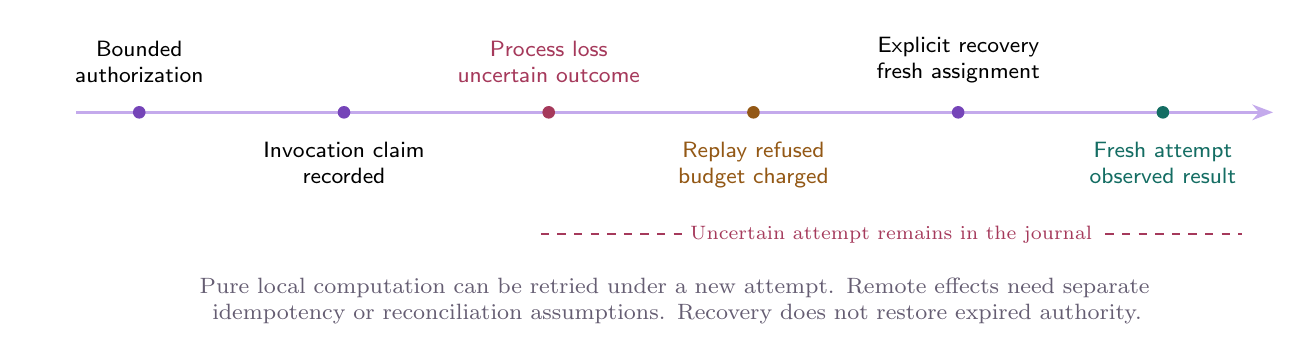
\begin{tikzpicture}[font=\sffamily\footnotesize,>=Stealth]
\draw[->,line width=1pt,draw=Lilac] (0,0)--(15.2,0);
\foreach \x/\col in {.8/Violet,3.4/Violet,6/Rose,8.6/Amber,11.2/Violet,13.8/Teal}{\fill[\col] (\x,0) circle(.08);}
\node[align=center,text width=2.6cm,anchor=south] at (.8,.25) {\mbox{Bounded}\\\mbox{authorization}};
\node[align=center,text width=2.6cm,anchor=north] at (3.4,-.25) {\mbox{Invocation claim}\\\mbox{recorded}};
\node[align=center,text width=2.6cm,anchor=south,text=Rose] at (6,.25) {\mbox{Process loss}\\\mbox{uncertain outcome}};
\node[align=center,text width=2.6cm,anchor=north,text=Amber] at (8.6,-.25) {\mbox{Replay refused}\\\mbox{budget charged}};
\node[align=center,text width=2.6cm,anchor=south] at (11.2,.25) {\mbox{Explicit recovery}\\\mbox{fresh assignment}};
\node[align=center,text width=2.6cm,anchor=north,text=Teal] at (13.8,-.25) {\mbox{Fresh attempt}\\\mbox{observed result}};
\draw[Rose,dashed,line width=.8pt] (5.9,-1.55)--(14.8,-1.55);
\node[text=Rose,font=\scriptsize,fill=white,inner sep=3pt] at (10.35,-1.55) {Uncertain attempt remains in the journal};
\node[text width=15.2cm,align=center,font=\footnotesize,text=Muted] at (7.6,-2.4) {Pure local computation can be retried under a new attempt. Remote effects need separate\\idempotency or reconciliation assumptions. Recovery does not restore expired authority.};
\end{tikzpicture}

% END input
}
\caption{The recovery timeline preserves the interrupted attempt. The companion includes both an injected lost-result boundary and a genuine subprocess-exit control; their scopes are reported separately.}
\label{fig:recovery}
\end{figure}

\begin{proposition}[Scoped duplicate suppression]
Assume a single authoritative durable journal, atomic persistence of an invocation claim before handler entry, no rollback to an earlier journal prefix, and enforcement of the attempt-scoped identity $(\text{institution},\text{job},\text{authorization},\text{invocation identifier})$ on every invocation. Then that same tuple cannot enter the handler twice through the dispatcher. This does not imply exactly-once completion or exactly-once external effects.
\end{proposition}
\begin{proof}
The first accepted invocation persists the claim before handler entry. Every later use sees an existing claim and is refused. If the first invocation dies before completion, refusal still prevents a second entry under that identity, while the completion status remains uncertain. A fresh authorization creates a different tuple even when its invocation-identifier string is reused; destination-side effect deduplication would require an additional assumption.
\end{proof}

A remote payment, actuator or service request would need a destination idempotency key, a queryable receipt or a reconciliation procedure, with a documented failure policy. None is exercised here. Calling a local numerical function again under a new research attempt is not evidence of safe repetition of an irreversible external action.

A hash-linked journal also has a trust boundary. Its signatures authenticate a key, not the human independence of its holder. A valid truncated prefix can evade detection without a separately retained head checkpoint. The companion's test identities are intentionally public fixtures: their purpose is to exercise source behavior, not to provide production authenticity.

\subsection{Capability packaging and succession}

A capability package contains executable code or a construction procedure, typed inputs and outputs, dependencies and versions, applicability limits, error/quality claims, provenance, qualification evidence and a finite rejection behavior. It is reusable only when the receiving mission can establish compatibility and afford the remaining checks. A package that cannot explain its domain is a cached answer with an uncertain meaning.

\begin{definition}[Transfer obligation]
For capability $C$ and successor mission $M'$, a transfer obligation is the set $T(C,M')$ of assumptions, interfaces, semantic checks and current permissions that must be re-established before use. Transfer is admissible only when every required obligation is discharged within $M'$'s constraints; retained evidence can discharge only obligations within its recorded scope.
\end{definition}

In the photometer, nuisance-basis construction and exact arithmetic machinery can transfer. A scalar estimator's output type and normalization certificate cannot certify a two-channel estimator. Fresh gain/reference observations and a new mission-specific error check remain necessary. The current execution grant also starts anew. The successor artifact links its parent by content and provenance without representing a parent acceptance as a present child acceptance.

\begin{figure}[htbp]
\centering\resizebox{.97\linewidth}{!}{
% BEGIN figures/lineage.tex
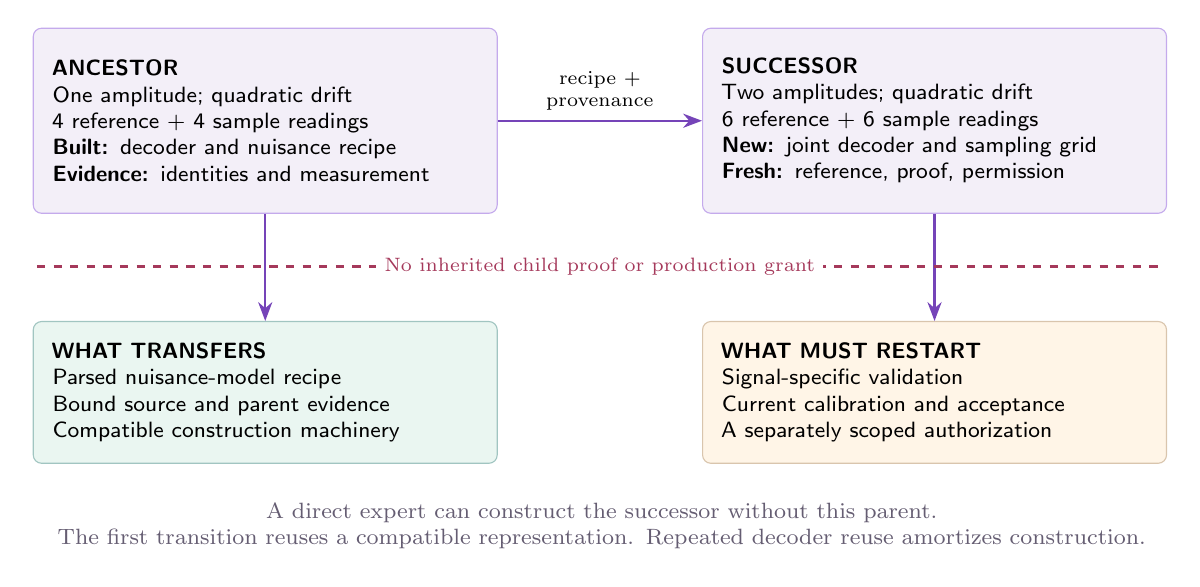
\begin{tikzpicture}[font=\sffamily\footnotesize,>=Stealth,
 box/.style={draw=Lilac,fill=Mist,rounded corners=3pt,text width=5.4cm,minimum height=2.35cm,align=left,inner sep=7pt},
 arr/.style={->,draw=Violet,line width=.85pt}]
\node[box] (parent) at (0,0) {\textbf{ANCESTOR}\\One amplitude; quadratic drift\\4 reference + 4 sample readings\\\textbf{Built:} decoder and nuisance recipe\\\textbf{Evidence:} identities and measurement};
\node[box] (child) at (8.5,0) {\textbf{SUCCESSOR}\\Two amplitudes; quadratic drift\\6 reference + 6 sample readings\\\textbf{New:} joint decoder and sampling grid\\\textbf{Fresh:} reference, proof, permission};
\draw[arr] (parent.east)--node[above,align=center,font=\scriptsize]{recipe +\\provenance}(child.west);
\node[box,fill=Mint,draw=Teal!40,minimum height=1.8cm] (stable) at (0,-3.45) {\textbf{WHAT TRANSFERS}\\Parsed nuisance-model recipe\\Bound source and parent evidence\\Compatible construction machinery};
\node[box,fill=Sand,draw=Amber!35,minimum height=1.8cm] (reset) at (8.5,-3.45) {\textbf{WHAT MUST RESTART}\\Signal-specific validation\\Current calibration and acceptance\\A separately scoped authorization};
\draw[arr] (parent)--(stable);
\draw[arr] (child)--(reset);
\draw[Rose,line width=1pt,dashed] (-2.9,-1.85)--(11.4,-1.85);
\node[font=\scriptsize,text=Rose,fill=white,inner sep=3pt] at (4.25,-1.85) {No inherited child proof or production grant};
\node[text width=14.3cm,align=center,font=\footnotesize,text=Muted] at (4.25,-5.15) {A direct expert can construct the successor without this parent.\\The first transition reuses a compatible representation. Repeated decoder reuse amortizes construction.};
\end{tikzpicture}

% END input
}
\caption{Capability lineage across a changed output contract. The parsed parent recipe is actually consumed at the new sampling grid. The scalar decoder and its current authorization are insufficient for the joint mission.}
\label{fig:lineage}
\end{figure}

Let $C_0$ be initial construction/qualification cost, $R_m$ the mission-relative reuse and requalification cost, $D_m$ the direct reconstruction cost, and $H_m$ harness overhead, all measured in a declared compatible resource coordinate. Reuse is cheaper in that coordinate only if
\begin{equation}
C_0+\sum_{m=1}^{n}(R_m+H_m)<\sum_{m=1}^{n}D_m.
\label{eq:breakeven}
\end{equation}
This inequality is a condition, not an assumed outcome. The study evaluates several resource coordinates separately. Unknown human construction and review time prevents a complete monetary conclusion even when a counted-operation inequality holds.

\subsection{What is established practice}

Durable workflows and retries, event logs, idempotency tokens, content-addressed builds, typed interfaces, independent validation and explicit access grants all have substantial precedents \cite{temporal,awsidempotency,buildsystems,pcc,prov,sqlite}. The present work uses those ideas and existing project code. Its claim is narrower: these mechanisms can make a capability transition inspectable enough to test whether the subsequent mission becomes feasible and whether reuse pays for itself. The scientific construction, strong alternatives and preserved failures supply the evidence for that claim.

% END input


% BEGIN sections/instrument.tex
\section{A photometer that becomes a different instrument}
\label{sec:instrument}

The experiment is a computational instrument emulator. It does not operate a physical detector. The quantities called readings below are counted simulated detector acquisitions; the exact-arithmetic work that designs an estimator is counted separately. The scenario is nevertheless a useful instrumentation problem: separate known modulated responses from an unknown drifting background and an uncertain gain.

\subsection{The declared measurement world}

For $n$ acquisition times and $p$ target channels, let
\begin{equation}
\mathbf y=gR\mathbf s+V_d\boldsymbol\beta+\mathbf e,
\qquad (V_d)_{ik}=t_i^k,\quad k=0,\ldots,d.
\label{eq:world}
\end{equation}
Here $\mathbf s\in[-1,1]^p$ is the unknown sample amplitude, $R\in\{-1,+1\}^{n\times p}$ is the controlled response pattern, $g\in[4/5,6/5]$ is the gain, $\boldsymbol\beta$ is an unrestricted polynomial background, and $|e_i|\leq\eta=1/500$. One mission's reference and sample share a gain. Their polynomial coefficients can differ arbitrarily. The drift order $d$ is an explicit world assumption, not something guaranteed by a good fit to a few observations.

We seek an executable estimator matrix $W\in\mathbb Q^{p\times n}$ satisfying
\begin{equation}
WV_d=0,\qquad WR=I_p.
\label{eq:identities}
\end{equation}
Then $W\mathbf y=g\mathbf s+W\mathbf e$: every declared nuisance polynomial disappears exactly in the model. For row $w_j$ of $W$, the remaining additive error is bounded by $\delta_j=\eta\|w_j\|_1$. This algebra is classical linear estimation and drift cancellation \cite{doiron,swanson}. The research constructs a finite program and tests its transfer, rather than claiming the algebra as new.

\begin{proposition}[Identifiability modulo nuisance]
An estimator satisfying Eq.~\eqref{eq:identities} exists if and only if the columns of $R$ are linearly independent modulo the column space of $V_d$, equivalently
\begin{equation}
\operatorname{rank}[V_d\;R]-\operatorname{rank}V_d=p.
\label{eq:rank}
\end{equation}
When $V_d$ has full column rank, this requires $n\geq d+1+p$.
\end{proposition}
\begin{proof}
If $Ra$ is in the nuisance space, any annihilator of that space maps it to zero. The identity $WR=I_p$ would map it to $a$, so only $a=0$ is allowed. Conversely, independence in the quotient lets one define a linear map that annihilates the nuisance space and maps each signal column to its corresponding coordinate; extending that map to the observation space gives $W$. With full nuisance rank, Eq.~\eqref{eq:rank} requires $d+1+p$ independent columns.
\end{proof}

The implemented finite constructor enumerates the declared response candidates, rejects deficient rank, and computes the target rows of $(B^TB)^{-1}B^T$ for $B=[V_d\;R]$ using rational arithmetic. The exhaustive policy minimizes maximum row $\ell_1$ norm over \emph{that finite candidate library}, breaking ties by total squared row norm and lexical order. It is not a globally optimal search over every physically possible instrument. The expert-coded comparator may stop at the first candidate that satisfies the mission's quality requirement; a mission that needs feasibility need not pay for exhaustive minimax design.

\subsection{The ancestor: one signal through quadratic drift}

The ancestor follows the actual revised Out-Learn construction \cite{outlearn}. At times $(0,2,3,5)$ with response $(1,1,-1,-1)^T$, use
\begin{equation}
w=\tfrac18(-1,5,-5,1).
\label{eq:ancestor}
\end{equation}
The row annihilates $1,t,t^2$ and maps the response to one. This creates a scalar measurement interface despite unknown quadratic background. It still needs calibration because multiplication by $g$ remains. Four reference readings and four sample readings produce one calibrated scalar mission. The ancestor package preserves the schedule, model, exact identities, implementation source and applicability; it is not a free certificate for a future rank-two task.

\subsection{The successor: two channels in one acquisition window}

The successor asks for two independent spectral amplitudes under a twelve-reading cap. Two separately calibrated uses of the four-reading scalar procedure would use sixteen readings. The new candidate uses six joint reference readings and six joint sample readings. Its pattern library contains balanced length-six sign vectors with first entry positive; each unordered pair is a candidate $R$. The output is a two-row estimator, not two copies of the old scalar answer.

The changed requirement makes the contribution visible. The retained exact solver and nuisance representation help construct the new instrument, but $W$, the signal interface and its current checks must change. A cubic-background successor needs yet another nuisance model; two channels with quartic drift are not identifiable from the declared six observations because $5+2>6$. Rank refusal is useful evidence: it establishes a finite limit rather than manufacturing a successful descendant.

The twelve-versus-sixteen contrast is conditional on \emph{separately calibrated sequential scalar procedures}. A more capable conventional joint design is allowed and expected to match the twelve-reading construction. The paper does not claim a universal lower bound of sixteen for all conventional approaches or attribute the joint algebra exclusively to the Harness.

\subsection{Fresh calibration and an explicit quality bound}

The reference uses known target amplitudes equal to one. After applying $W$, reference coordinate $r_j$ bounds the shared gain by $[r_j-\delta_j,r_j+\delta_j]$. The mission intersects all these intervals with $[g_{\min},g_{\max}]$. An empty intersection is a rejection. Each sample coordinate $z_j$ produces a signal interval by dividing $[z_j-\delta_j,z_j+\delta_j]$ by the positive gain interval and intersecting with $[-1,1]$. The reported estimate is the interval midpoint.

With $\delta=\eta\max_j\|w_j\|_1$, $\delta\leq g_{\min}/2$, and the declared amplitude clipping, a conservative worst-case interval radius is
\begin{equation}
\rho\leq \frac{2\delta}{g_{\min}+2\delta}.
\label{eq:radius}
\end{equation}
One way to see the bound is to write the widest possible gain interval as $[a,a+2\delta]$, $a\geq g_{\min}$. If the sample interval straddles zero, its radius is at most $\delta/a\leq2\delta/(a+2\delta)$ under the stated condition. Otherwise, for nonnegative sample center, the signal interval width increases until its upper end first reaches one. At that point the center is $a-\delta$ and half the clipped interval width is $2\delta/(a+2\delta)$. Beyond it, clipping decreases the width. The negative case is symmetric. A narrower gain interval or smaller coordinate error cannot enlarge this upper bound. Every accepted design in this study satisfies the small-noise condition. In general the clipped bound is $\min\{1,\max[2\delta/(g_{\min}+2\delta),\delta/g_{\min}]\}$ \cite{outlearn}. The argument depends on positive bounded gain, bounded additive noise, the shared-gain reference assumption and the amplitude range; relaxing them requires a different bound.

The frozen acceptance threshold is $\rho\leq1/50$ and actual absolute signal error at most $1/50$. The primary outcome requires both the executable validator's acceptance and simulator truth inside the reported interval. We therefore distinguish \emph{validator-accepted} from \emph{oracle-qualified}; their disagreement is a central failure result, not a terminological inconvenience.

\subsection{What the instrument cannot know}

Suppose the sample includes unmodeled interference $R\mathbf b$. Then
\begin{equation}
gR\mathbf s+R\mathbf b+V_d\boldsymbol\beta
=gR(\mathbf s+\mathbf b/g)+V_d\boldsymbol\beta.
\label{eq:indistinguishable}
\end{equation}
Within this measurement scheme, the interference is indistinguishable from a changed target amplitude. The rank certificate and nuisance identities can remain valid while the scientific answer is wrong. Likewise, a gain change between reference and sample invalidates the calibration assumption. No amount of signed journaling resolves this observational ambiguity. A physical deployment would require independent observables, stronger controls, or additional model validation. The companion preserves such failures visibly.

% END input


% BEGIN sections/protocol.tex
\section{Frozen experimental protocol and fair alternatives}
\label{sec:protocol}

The prospective protocol was written and hashed before the main evaluation. Its identity, original bytes and checkpoint are included in the package. The protocol fixes the candidate library, noise and gain ranges, acceptance threshold, generator seeds, mission order, budgets and stopping rule. It is a local preregistration checkpoint, not a registration with an independent external registry. Any implementation correction is retained separately with its chronology; later reruns are not relabelled unseen confirmation.

\subsection{Primary study}

Four held-out campaigns use seeds 73001--73004 and 48 ordered missions each. Mission zero is the scalar quadratic ancestor. Subsequent blocks mix joint quadratic, joint quadratic, joint cubic and scalar quadratic requirements. Each method sees identical hidden simulator draws: amplitudes in $[-.9,.9]$, gain in $[.8,1.2]$, independently drawn polynomial coefficients for reference and sample, and additive noise bounded by .002. Construction sees the declared task family, not those outcome draws. This is within-family generalization to new parameters and a designed semantic transition, not open-domain autonomous scientific discovery.

The shared per-campaign budget is the vector
\begin{equation}
B=(800\ \text{simulated readings},\;2{,}000{,}000\ \text{counted rational operations},\;48\ \text{missions}).
\label{eq:budget}
\end{equation}
The counter checks a resource reservation before it occurs. Exceeding any component stops the ordered campaign; a method cannot skip the stopped mission to collect easier later successes. Failed construction work remains charged. The primary metric is the number of oracle-qualified missions completed before exhaustion. All ancestor costs are included.

\begin{table}[htbp]
\centering\small
\begin{tabularx}{\linewidth}{P{.22\linewidth}Y Y}
\toprule
\textbf{Method} & \textbf{Construction and reuse} & \textbf{What the comparison asks}\\
\midrule
Harness reuse & Exhaustive finite design; cache compatible artifacts; fresh reference and validation for every mission. & Does the capability transition operate with explicit receipts and transfer obligations?\\
Conventional reuse & The same design code, compatible cache, persistence eligibility and validators. & Does a competent ordinary workflow achieve the same scientific outcomes and costs?\\
Expert-coded construction & First feasible exactly checked design from the same candidates; cache and validators retained. & Does a cheaper sufficient design beat exhaustive optimization?\\
Rebuild search & The same exhaustive constructor and checks, with reconstruction per mission. & What is lost when reusable construction is deliberately discarded?\\
\bottomrule
\end{tabularx}
\caption{The strongest ordinary comparator receives reuse. Rebuilding is an ablation, not a stand-in for conventional engineering. The expert is a supplied deterministic program, not an observed human participant.}
\label{tab:comparators}
\end{table}

The scientific reuse policies deliberately share their numerical functions. Equality is meaningful: it attributes any science-level benefit to the instrument and reuse rather than to a brand or a workflow label. The separate orchestration comparison uses actual local durable implementations, the same scientific tasks and validators, and reports its implementation and matching limits. We do not describe that comparison as a benchmark of Temporal or another unexecuted commercial workflow engine.

\subsection{Full costs without invented exchange rates}

The cost ledger reports construction, execution and fresh qualification rational operations; simulated detector acquisitions; measured wall and process CPU time; cache hits; failures; recovery charges; and intervention records. The counted arithmetic includes rational additions, subtractions, multiplications and divisions in declared kernels. Candidate generation, comparisons, hashing, serialization and interpreter overhead appear in CPU/wall time, not in the arithmetic count. A counted rational operation has input-dependent real cost, so the count is neither a hardware instruction count nor a portable latency estimate.

The resource coordinates are not summed into an artificial total. The complete measured pipeline cost is reported \emph{within each coordinate}. No paid service or financial transaction is invoked; the environment's allocation price, embodied authoring effort and long-term maintenance are unknown. No human participants are timed. Scripted recovery decisions are distinguished from actual operator intervention. Unknown labor is not set to zero, and modeled savings are not realized profit.

\subsection{Negative controls, ablations and stopping}

The frozen controls include unmodulated confounding, collinear channel patterns, too much nuisance dimension for the acquisition window, scalar-to-joint misuse, stale nuisance proof, a corrupted estimator, stale gain, signal-shaped interference and an insufficient resource cap. The first group tests rejection; the last model violations test what the validator can miss. Stage-linked structural probes inspect these obligations. The response-only estimator, separate-scalar plan and no-cache rebuild alter specific computations; the other negative controls do not establish causal necessity of each named callback. For example, removing a separate rank check does not prevent the matrix inverse from independently failing closed on a singular design.

Runtime controls separately examine duplicate invocation, interrupted execution, exact-attempt recovery, expiry, cancellation, source binding, dependency revocation and descendant state. They use the released dispatcher and explicit local fixtures. A test that refuses an invalid action is an observed source behavior. It is not a proof against every crash schedule, concurrent actor, malicious plugin or compromised host.

The protocol's main stopping rule forbids post-result threshold tuning. All paired campaign outcomes are published. Timings are descriptive measurements on the recorded host, and exact scientific outcomes are verified by deterministic reproduction. The load experiment varies offered work with a bounded local concurrency model; no measured local throughput is extrapolated to a production fleet or to physical acquisitions.

% END input


% BEGIN sections/results.tex
\section{Results: a new capability, a tie, and a cheaper expert}
\label{sec:results}

\subsection{The constructed change in feasibility}

The finite search constructs the quadratic-background joint decoder
\begin{equation}
R=\begin{bmatrix}1&1\\-1&-1\\-1&1\\1&-1\\1&1\\-1&-1\end{bmatrix},\qquad
W=\frac1{16}\begin{bmatrix}2&-2&-4&4&2&-2\\1&-3&4&-4&3&-1\end{bmatrix},
\quad t=(0,1,2,3,4,5).
\label{eq:joint}
\end{equation}
Both rows annihilate the quadratic nuisance basis and satisfy $WR=I_2$. Both have $\ell_1$ norm one, giving the conditional calibrated bound $1/201\approx.004975$. For any normalized row with a sign-valued target response, $1=|wr|\leq\|w\|_1$; these rows attain that lower bound for the declared response/noise model. This does not prove global optimality over hardware, time or other acquisition models.

The constructed artifact is materially different from Eq.~\eqref{eq:ancestor}: it returns two amplitudes from one six-reading block. A fresh six-reading reference plus six-reading sample fits the twelve-reading successor cap. The separate-scalar control spends eight readings on the first channel and cannot reserve the second eight. The primary conventional and expert methods are allowed the joint program and also fit the cap. The feasibility result is therefore relative to the scalar incumbent, not a monopoly of the Harness.

The child actually parses a source-bound symbolic nuisance recipe constructed by the ancestor and evaluates it on the new grid. The scalar-to-dual path counts 47,157 rational operations, compared with 47,108 for a fresh direct dual construction: a 49-operation inheritance overhead. Including the ancestor, the two-mission scientific demonstration uses 47,956 operations and twenty simulated readings. The first transition is a preserved loss in counted cost; compatible decoder reuse over later missions is a separate result.

\subsection{Primary held-out mission coverage}

All four methods qualify 48 of 48 missions in each of the four campaigns, for 192 of 192 per method and 768 accepted method--mission observations in total. All use 2,112 simulated readings per method. No method hits the preregistered acquisition or operation ceiling. Exhaustive rebuild uses 1,988,316 operations per campaign, just below the fixed 2,000,000 limit. We retain that outcome: \textbf{the primary coverage advantage is zero at the frozen budget.}

\begin{table}[htbp]
\centering\small
\begin{tabularx}{\linewidth}{Y r r r r}
\toprule
\textbf{Scientific policy} & \textbf{Qualified} & \textbf{Rational ops} & \textbf{Readings} & \textbf{Max error}\\
\midrule
Harness reuse & 192/192 & 609,524 & 2,112 & .00328335\\
Conventional reuse & 192/192 & 609,524 & 2,112 & .00328335\\
Expert-coded sufficient design & 192/192 & 169,732 & 2,112 & .00336635\\
Exhaustive rebuild & 192/192 & 7,953,264 & 2,112 & .00328335\\
\bottomrule
\end{tabularx}
\caption{All four paired held-out campaigns, including ancestor construction and fresh numerical validation. The error threshold is .02. These counts describe the scientific callbacks; actual orchestration overhead is measured separately, not hidden inside an invented operation exchange rate.}
\label{tab:primary}
\end{table}

Harness and conventional reuse match every scientific receipt and counted cost in all four campaigns. Their different wall times are host variation over identical scientific policies, not evidence of a scientific speedup. The expert-coded sufficient policy uses 72.15\% fewer counted operations than the exhaustive reuse policies and still meets the same quality criterion. Its maximum observed interval radius is .008738, compared with .005987 for exhaustive reuse; the tolerance is .02. Paying for tighter estimates was unnecessary for qualification in these missions.

Exhaustive reuse uses 92.34\% fewer counted operations than exhaustive reconstruction, including the other numerical phases. That comparison demonstrates amortization against discarded construction, not superiority over competent cached engineering. Cache-enabled methods each construct twelve capabilities across the four independently cold campaigns and reuse them 180 times. Rebuild constructs a capability for every one of the 192 missions.

\begin{figure}[htbp]
\centering
% BEGIN figures/comparison.tex
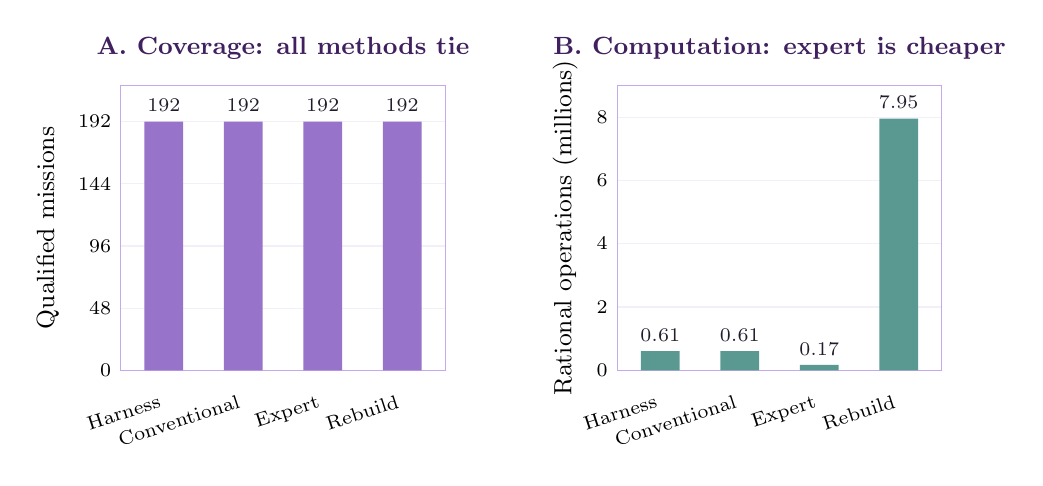
\begin{tikzpicture}
\begin{axis}[width=.47\linewidth,height=5.2cm,ybar,bar width=14pt,symbolic x coords={Harness,Conventional,Expert,Rebuild},xtick=data,x tick label style={font=\scriptsize,rotate=18,anchor=north east},y tick label style={font=\scriptsize},ylabel={Qualified missions},ylabel style={font=\small},ymin=0,ymax=220,ytick={0,48,96,144,192},axis line style={draw=Lilac},tick style={draw=none},ymajorgrids=true,grid style={draw=Mist},nodes near coords,nodes near coords style={font=\scriptsize,text=Ink},title={\textbf{A. Coverage: all methods tie}},title style={font=\small,text=Cosmic},enlarge x limits=.18]
\addplot[fill=Violet!75,draw=none] coordinates {(Harness,192)(Conventional,192)(Expert,192)(Rebuild,192)};
\end{axis}
\begin{axis}[at={(.52\linewidth,0)},anchor=south west,width=.47\linewidth,height=5.2cm,ybar,bar width=14pt,symbolic x coords={Harness,Conventional,Expert,Rebuild},xtick=data,x tick label style={font=\scriptsize,rotate=18,anchor=north east},y tick label style={font=\scriptsize},ylabel={Rational operations (millions)},ylabel style={font=\small},ymin=0,ymax=9,ytick={0,2,4,6,8},axis line style={draw=Lilac},tick style={draw=none},ymajorgrids=true,grid style={draw=Mist},nodes near coords,nodes near coords style={font=\scriptsize,text=Ink,/pgf/number format/fixed,/pgf/number format/precision=2},title={\textbf{B. Computation: expert is cheaper}},title style={font=\small,text=Cosmic},enlarge x limits=.18]
\addplot[fill=Teal!70,draw=none] coordinates {(Harness,.609524)(Conventional,.609524)(Expert,.169732)(Rebuild,7.953264)};
\end{axis}
\end{tikzpicture}
\par\vspace{7mm}
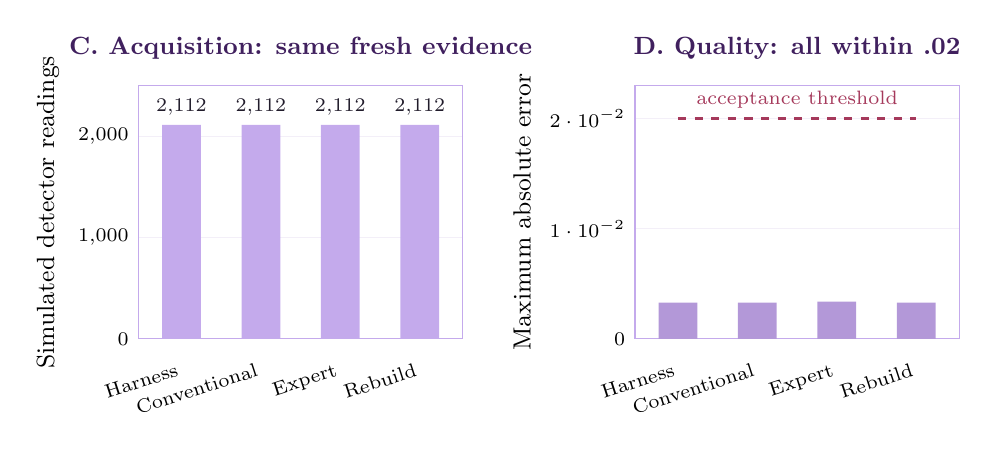
\begin{tikzpicture}
\begin{axis}[width=.47\linewidth,height=4.8cm,ybar,bar width=14pt,symbolic x coords={Harness,Conventional,Expert,Rebuild},xtick=data,x tick label style={font=\scriptsize,rotate=18,anchor=north east},y tick label style={font=\scriptsize},ylabel={Simulated detector readings},ylabel style={font=\small},ymin=0,ymax=2500,ytick={0,1000,2000},scaled y ticks=false,axis line style={draw=Lilac},tick style={draw=none},ymajorgrids=true,grid style={draw=Mist},nodes near coords,nodes near coords style={font=\scriptsize,text=Ink},title={\textbf{C. Acquisition: same fresh evidence}},title style={font=\small,text=Cosmic},enlarge x limits=.18]
\addplot[fill=Lilac,draw=none] coordinates {(Harness,2112)(Conventional,2112)(Expert,2112)(Rebuild,2112)};
\end{axis}
\begin{axis}[at={(.52\linewidth,0)},anchor=south west,width=.47\linewidth,height=4.8cm,ybar,bar width=14pt,symbolic x coords={Harness,Conventional,Expert,Rebuild},xtick=data,x tick label style={font=\scriptsize,rotate=18,anchor=north east},y tick label style={font=\scriptsize},ylabel={Maximum absolute error},ylabel style={font=\small},ymin=0,ymax=.023,ytick={0,.01,.02},scaled y ticks=false,axis line style={draw=Lilac},tick style={draw=none},ymajorgrids=true,grid style={draw=Mist},title={\textbf{D. Quality: all within .02}},title style={font=\small,text=Cosmic},enlarge x limits=.18]
\addplot[fill=Violet!55,draw=none] coordinates {(Harness,.00328335)(Conventional,.00328335)(Expert,.00336635)(Rebuild,.00328335)};
\draw[Rose,dashed,line width=.9pt] (axis cs:Harness,.02)--(axis cs:Rebuild,.02) node[pos=.5,above,font=\scriptsize,text=Rose]{acceptance threshold};
\end{axis}
\end{tikzpicture}

% END input

\caption{The comparison preserves both ties and losses. Qualified coverage and simulated readings are equal at the frozen budget. Counted numerical work favors the expert-coded sufficient design, while all quality measurements remain below the threshold. These are separate resource/quality coordinates, not a single utility score.}
\label{fig:comparison}
\end{figure}

\subsection{Where the numerical work goes}

For Harness reuse, the complete 609,524 counted-operation ledger includes 465,524 construction operations, 43,536 identification operations, 18,480 nuisance-representation operations, 16,080 rank/interface operations, 51,936 fresh requalification operations and 13,968 execution operations. Conventional reuse has the same ledger. The expert reduces construction to 25,732 operations; its other phase totals are identical. Rebuild spends 7,809,264 on construction.

These counts include the numerical costs of the stage callbacks, but not every machine instruction. Evaluation-world generation, truth checks, hashing, integer budget decisions, serialization and the interpreter contribute to measured CPU/wall time instead. Primary aggregate process CPU times were approximately 1.060 s for Harness scientific policy, 1.085 s for conventional reuse, .680 s for the expert and 7.187 s for rebuild on the recorded host. They are descriptive single-process measurements, not portable service guarantees. Runtime orchestration and recovery receive separate measurements below.

The non-construction ledger totals 144,000 operations per method. It would be misleading to advertise only the cheap final dot product while omitting model construction, fresh validation and ancestor costs. It would also be misleading to call 609,524 rational operations a price or to add them to 2,112 simulated detector acquisitions as though they were the same resource.

\subsection{Failures the validator detects, and failures it misses}

Seven of the nine scientific negative controls produce the intended refusal: unmodulated confounding, collinear channels, excessive nuisance dimension, scalar-as-dual reuse, stale nuisance scope, corrupted weights despite a recomputed hash, and an eleven-reading cap. All stop before detector acquisition. Their shared control-construction cost is retained separately, rather than credited as free testing.

Two controls are accepted internally while failing against simulator truth. Changing gain from .8 during reference to 1.2 during sample yields absolute errors of approximately .199255 and .099629; the declared .02 tolerance is violated. Signal-shaped interference causes a first-channel error of approximately .100005 while the algebra and reported narrow interval remain internally consistent. These are failures of the world assumption/observability boundary, not caught scientific successes. The raw results preserve both \code{accepted:true} and \code{oracle\_qualified:false}.

The response-only estimator without nuisance modeling incurs a .5 error on one controlled sample. The separate-scalar plan exceeds the successor's cap. The no-cache comparison preserves quality but repeats construction. The remaining stage-linked probes show applicability/refusal obligations; they do not prove that all seven named callbacks are causally indispensable. The solver's independent singularity rejection, for example, can protect a path even without a separate earlier rank check.

A correction-and-recovery scientific sequence retains the accepted quadratic instrument, refuses a corrupted candidate, and constructs and freshly qualifies a cubic-background successor. The incremental correction-and-recovery sequence costs 70,478 counted operations and twenty-four simulated readings; the shared control construction of 46,992 operations is separately retained. The rejected history is not rewritten. The scientific sequence is separate from process-crash recovery in the released runtime.


% BEGIN sections/runtime_results.tex
\subsection{Actual dispatcher execution and recovery}

The final released-source nominal run completes fourteen real stage callbacks across the scalar ancestor and joint successor, producing 106 verified journal events. Both receive fresh local qualification and separate sandbox inspection grants. Attempting to record the ancestor's proof as the child's proof is refused. The artifact auditor verifies all fourteen accepted work receipts and their retained outputs without importing the runtime or scientific constructor.

The crash scenario injects loss after the ancestor's pure measurement calculation but before result retention. The reopened journal refuses the same invocation identity. A scripted controller records recovery and issues a new assignment; the original uncertain attempt remains. The final history has 112 events and fourteen accepted stage receipts. The test apparatus observes an extra eight simulated readings and 82 rational operations, bringing the scientific total to twenty-eight readings and 48,038 operations. The runtime correctly leaves the lost attempt's actual cost unknown and charges its reservation; the observer's knowledge is not silently substituted into that journal.

The impossible-successor scenario requests two channels plus quartic nuisance within six observations. The ancestor remains accepted, the child is refused at design, and its three downstream stages remain unrun. The history contains 84 events and ten accepted stage receipts. Its retained scientific counter is 1,617 operations \emph{plus unknown rejected-design work}; it is not a complete numerical cost. Measured run time and the conservatively charged runtime reservation retain the execution cost boundary. Only the ancestor's eight detector readings occur.

The original runtime control campaign matches all thirteen predeclared expected behaviors. This includes a genuine subprocess exit with code 23 after a durable invocation claim, replay refusal, exact-attempt recovery, dependency revocation, changed output binding, expired assignment, fresh descendant proof/grant boundaries and budget overrun. It also deliberately includes a \emph{miss}: a generic runtime accepts a physically false assertion when its configured acceptance role signs it. Thus ``13/13 expectations matched'' is not ``13 security defenses succeeded.''

Two separately frozen supplemental controls verify STOP during computation and authorization expiry after computation. In both, the callback may finish, but the post-handler boundary suppresses its output and preserves a failed invocation requiring explicit recovery. The tests establish cooperative boundary refusal, not asynchronous preemption or a hard real-time execution deadline. The STOP fixture directly invokes the host's durable local flag; remote authentication is not exercised. Recovery does not clear STOP or restore expired permission.

Tampered event content is rejected. A valid truncated journal prefix verifies by itself and is rejected only when compared with the separately retained head checkpoint. This is the intended custody limit. Three public RFC test-vector signatures, the exact fixture schema and all eleven vendored runtime file identities also pass the independent fixture audit. These are local source and representation checks, not secret-key custody or deployed identity assurance.

\subsection{Load, latency and oversight cost}

A second protocol was frozen before any load timing. It compares the actual released dispatcher with a competent direct durable loop using the same seven callbacks, cold-per-batch compatible cache, scientific validators, typed receipts, public fixture signatures, SQLite journal and artifact persistence. The direct loop enforces the nominal sequence, exact source/terms, expiry, call ceiling and invocation replay guard. It deliberately omits graph-wide role separation, descendant admission/authority, revocation propagation and recovery. It is a nominal-workflow ablation, not a demonstrated equivalent production engine.

There are three paired repetitions at batch sizes one, eight and thirty-two, with alternating method order and one sequential worker. All missions are available at batch start. Eighteen batches complete with 246 of 246 qualified mission executions and zero observed failures. All nine pairs match on scientific context, detector counts and rational-operation counts. The reported throughput includes fixture initialization, construction, cache and artifact writes, final journal verification, event export and checkpoint retention. Imports and the final summary write are excluded consistently.

\begin{table}[htbp]
\centering\small
\begin{tabularx}{\linewidth}{r Y r r r}
\toprule
\textbf{Queued} & \textbf{Implementation} & \textbf{Missions/s} & \textbf{Service median (s)} & \textbf{Service p95 (s)}\\
\midrule
1 & Alpha dispatcher & .868 & 1.097 & 1.097\\
1 & Direct durable loop & 11.455 & .070 & .070\\
8 & Alpha dispatcher & .765 & 1.255 & 1.408\\
8 & Direct durable loop & 8.221 & .105 & .153\\
32 & Alpha dispatcher & .816 & 1.149 & 1.322\\
32 & Direct durable loop & 9.342 & .097 & .144\\
\bottomrule
\end{tabularx}
\caption{Medians of three per-repeat summaries; p95 uses the nearest-rank rule within each repeat, followed by the median across repeats. These are not pooled percentiles. One local sequential worker is tested; increasing the batch changes queue length, not concurrency.}
\label{tab:load}
\end{table}

The direct loop wins the measured nominal overhead comparison. At thirty-two missions the median full batch time is 39.202 s for Alpha versus 3.425 s for the direct loop; the median of per-repeat queue-inclusive p95 completion times is 36.569 versus 3.109 s. Both perform 136,749 scientific rational operations and 320 simulated readings per batch. Alpha retains 1,442 events compared with 770 for the narrower loop. Its median retained artifact volume before summary is approximately 82.15 MB versus 10.03 MB. Those histories include different lifecycle detail; they are not equally compact representations of all the same governance features.

The measured cost makes the word ``thin'' an architectural description, not a demonstrated latency advantage. A practical deployment should decide which obligations justify that overhead, improve representation/verification costs where safe, and requalify the changed implementation. The study performs no such post-result optimization and preserves the slower result. Two separate post-measurement direct-loop checks refuse replay and request-payload rebinding without callback re-entry or history change; they do not supply missing governance equivalence.

There are no runtime human prompts in the scripted measurements. This does not measure authoring or oversight labor. The crash scenario requires one scripted recovery decision; an actual operator's time and judgment are unknown. The load results describe one host and do not establish a concurrency scaling law, independent reviewer capacity or production Fleet throughput.

% END input


\subsection{Conditions supported by the experiment}

The study supports reuse when the retained representation is compatible, the exact artifact survives integrity checks, fresh calibration and mission validation remain affordable, and repeated construction is a material cost. It does not support a blanket advantage over a competent workflow or a sufficient expert. Under the main resource vector, all methods have equal useful coverage; the most efficient sufficient constructor is the expert-coded reference. The Harness's distinct measured value is inspectable lifecycle behavior, for which its overhead and trust assumptions must be judged explicitly.

% END input


% BEGIN sections/system.tex
\section{The real system and its integration boundaries}
\label{sec:system}

The source and ownership audit was refreshed on 24 October 2026 against all four repositories and Alpha coordination issue 4850. The audit records exact commits, public release metadata, adapter paths and the current receiving-owner boundary \cite{alpha_source,jobs_source,manager_source,fleet_source,coordination}. It does not reinterpret a release label as execution of this new scientific adapter.

\begin{table}[htbp]
\centering\small
\begin{tabularx}{\linewidth}{P{.18\linewidth}P{.22\linewidth}Y}
\toprule
\textbf{System} & \textbf{Observed source/release} & \textbf{Evidence in this edition}\\
\midrule
AGI ALPHA & Main \code{031bdb5d}; public v1.41.0 & Released dispatcher source executed locally through a byte-pinned dependency closure. Manual public-fixture bootstrap; official installed initializer not run.\\
AGI Jobs v0 & Main \code{9983478d}; rc.20 product \code{f7c00e66} & Source inspection of the AGIALPHA18 admission route. This instrument is not newly admitted or settled through it.\\
AGI Job Manager & \code{c5958eae}; v1.20.1 & Source inspection of the distinct USDC6 route. No fresh Alpha 1.41 consumer acceptance claimed.\\
AGI Fleet Linux & Main \code{45759fb0}; historical v1.1.4 qualification & Source and ownership audit. Current combined integration candidate remains separately held; no scientific worker provisioned here.\\
\bottomrule
\end{tabularx}
\caption{Versions observed for this research audit. Full commit identities and public source URLs are in the package. Source execution, installed-package acceptance and deployed behavior are separate evidence levels.}
\label{tab:systems}
\end{table}

\subsection{The executed adapter}

The adapter calls \code{JobDispatcher.execute\_tool} with a locally installed handler and retained result bytes. It uses the released Journal, SuccessorStore, TrustRegistry, JobContract, ExecutionAuthorization, JobResult, ProofReceipt and AuthorityEnvelope mechanisms. It supplies the scientific callbacks through that seam. No production runtime module or held Harness overlay is modified.

The runtime's normal initializer creates local signing material and an API token. This writing brief requests no new credentials, so the research runner instead opens a deliberately public, manually prepared fixture journal using published RFC 8032 test vectors \cite{rfc8032}. The unchanged runtime still verifies signatures and roles, but anyone possessing the public fixtures can sign them. This is source-level behavioral evidence, not a production identity or authentication deployment. The isolated temporary journal is destroyed after export; exported events, public identities, source hashes and head checkpoints remain. No service account, wallet or chain connection is created.

The independent artifact auditor is a separate implementation that does not import the instrument constructor or the runtime's verification functions. It recomputes rational cancellation identities, calibration intervals and retained-output bindings, and verifies journal and role signatures against the public fixture keys. This is algorithmic separation under one research controller. It is not an independent organization, external certification or an audit of the cryptographic libraries.

\subsection{What remains outside the executed path}

The separately held Harness PRs 4863 and 4865 are not adopted. The current coordination record retains an unknown terminal result for configured review 6345107482 and a distinct merge denial 6347342683. The prepared current-main composition and its previously retained local regressions do not remove those restrictions. The existing release owners retain that lane.

Fleet's combined candidate \code{d0d4459b} likewise remains a separate owner/restriction decision. The accepted connected API history recorded by the coordinator uses Alpha 1.39, Jobs rc.20 and Manager 1.20.1; it is not an accepted Alpha 1.41 or four-installed tuple. The paper does not silently repin these consumers. Source inspection supplies an interface map, while this new photometer's Jobs, Manager and Fleet execution entries remain \status{NOT RUN}.

The existing publication coordinator owns shared catalogue edits, merge and Pages publication. This research delivers a new versioned manuscript and companion for that owner. A downloadable file, source branch or draft review is not a deployed website. Original research editions and their historical URLs remain separate.

\subsection{Five contracts, only their verified utility}

The five Alpha contracts are inspected at the same frozen Alpha commit. Table~\ref{tab:contracts} describes code-derived functions, not calls made by the scientific demonstration. A commitment can identify an exact mission artifact; it does not establish demand, profit, independent acceptance, or ownership of an entire opportunity.

\begin{table}[htbp]
\centering\small
\begin{tabularx}{\linewidth}{P{.21\linewidth}Y Y}
\toprule
\textbf{Contract} & \textbf{Verified source function} & \textbf{Possible harness relation}\\
\midrule
AscensionAccess & Live ENS/wrapper ownership plus an expiring governor admission for the declared role. & Optional eligibility gate. A role grant is not scientific competence or universal task authority.\\
NovaSeed & Immutable capsule, plan and evidence commitments; bounded job count; optional parent ownership link. & Commit to a source-bound mission package and ancestry. Commitment truth and successor qualification remain external.\\
AscensionRiskOracle & Staked eligible reviewer attestations, capacity locks and owner-bound time-limited risk decisions. & Optional risk/admission evidence. Different addresses do not establish independent organizational review.\\
AscensionJobMarket & Bounded posting, bidding, award, three reserved validators, two-vote outcome, deadlines and payout/refund branches. & Optional bounded work and settlement interface. A vote quorum does not automatically validate a measurement.\\
AscensionMark & Bounded funding lots, buy/sell/transfer, threshold transition, Merkle-plan-restricted job routing and unused-fund recovery. & Optional plan-bound funding mechanism. Tokenized participation is not a guaranteed return.\\
\bottomrule
\end{tabularx}
\caption{Source-derived mapping of the five-contract suite. The package includes exact file hashes and relevant source locations. No contract transaction, local EVM campaign, deployed read or real settlement is performed in this edition.}
\label{tab:contracts}
\end{table}

The Access roots in this suite are \code{*.alpha.agi.eth} for Business, \code{*.alpha.agent.agi.eth} for Agent and \code{*.alpha.club.agi.eth} for Validator. These source rules must not be confused with other repositories' ENS roles. NovaSeed's evidence hash and plan root are commitments, and parent token ownership is checked at sealing time; neither implies inherited current proof.

RiskOracle rechecks eligible positive signers and current owner identity for its green decision. JobMarket binds work to a specification hash, reserves eligible reviewers and distinguishes late execution from missing review, with different refund/slashing consequences. AscensionMark restricts routed jobs to the committed plan leaves. These mechanisms can make a future work relationship inspectable, provided a scientific validator is correctly attached and the application has current permission. None supplies the missing photometer validation merely by involving a token.

The shared Alpha token base requires canonical \$AGIALPHA with 18 decimals and checks exact token receipt/payment and burn behavior. Manager's USDC6 route is separate. A future application could place the paper's source-bound artifact commitment in a bounded job specification and reference the resulting evidence in a seed or risk decision. This paper supplies no funded offer, signed transaction or settlement result. It deliberately avoids adding transactions to make every contract appear utilized.

\subsection{A source receipt is not a deployment claim}

We use six explicit labels: source-derived inspection; local execution; installed-package execution; local EVM execution; read-only deployed observation; and real settlement. This study supplies the first two. The five contracts supply source-derived design constraints, not a seventh hidden execution layer. Public product releases remain their own evidence, with their own exact versions and accepted scope.

% END input


% BEGIN sections/discussion.tex
\section{What the results do and do not establish}
\label{sec:discussion}

The positive scientific result is a constructed change in the instrument's useful interface. One calibrated amplitude becomes two jointly identifiable amplitudes under the stated acquisition cap. The artifact is executable and its constraints are inspectable. The positive engineering result is that the existing dispatcher can preserve the work, source, attempts and qualification decisions while refusing several forms of invalid reuse.

The competent conventional workflow shares the same scientific outcome. That result is essential. Ordinary caching and validation are available to conventional engineering; removing them would mistake a weak baseline for a contribution. The expert-coded policy also shows that optimizing beyond the acceptance requirement can consume unnecessary construction work. A system organized around productive capability should be able to accept this comparator win and retain the sufficient design.

\subsection{Related work: reuse, evidence and execution}

Durable workflow systems already distinguish recorded orchestration from activities that may be retried; idempotent APIs bind repeated requests to an explicit identity \cite{temporal,awsidempotency}. RIFL combines durable completion records, request identity and defined retention assumptions to obtain linearizable operations in its system \cite{lee_rifl2015}. These precedents motivate the Harness's conservative treatment of uncertain outcomes. Its invocation journal supplies a scoped duplicate-entry guard; an external destination still needs its own effect and reconciliation contract.

Dependency-sensitive reuse is established in build systems and incremental computation. \emph{Build Systems \`a la Carte} separates scheduling decisions from decisions about whether a task must be rebuilt, and analyzes the dependencies needed for correct reuse \cite{buildsystems}. The present cache follows that engineering tradition. The additional experimental question is what remains reusable when the scientific output contract itself changes, and whether compatibility checks, fresh qualification and orchestration leave any net benefit. The conventional comparator receives ordinary caching precisely because that mechanism is established practice.

Certifying algorithms pair computed results with witnesses that a checker can inspect, while proof-carrying code makes compliance with a consumer's stated policy explicit \cite{mcconnell_certifying2011,pcc}. The photometer's cancellation and normalization identities provide small checkable witnesses in this spirit. They certify a conditional mathematical claim, while a signed work receipt attributes an acceptance decision. W3C PROV supplies a vocabulary for entities, activities, agents and derivations \cite{prov}; recording such provenance does not establish the truth of a physical model or confer current authority.

Drift-eliminating calibration and filtered comparison measurements also predate this study \cite{doiron,swanson}. The new experiment connects a constructed change in that instrument's output interface to explicit transfer obligations and an existing durable runtime. Its evidence includes the conventional tie, the cheaper sufficient constructor, the first-transition inheritance loss and the slower governed execution path. Those observations define the contribution more precisely than treating familiar mechanisms as novel because they appear in an agent workflow.

\subsection{Inheritance is an option with a price}

The first scalar-to-joint transition does not establish a cost advantage from parent inheritance. The ancestor contributes a constructed symbolic nuisance recipe, which the child verifies and evaluates at its new sampling grid. This is actual representation and provenance reuse. The generic solver was preexisting supplied code, and the child constructs a new decoder. A direct expert can build that decoder without the ancestor; parent-integrity checks add work. The measured savings against reconstruction arise when subsequent compatible missions reuse accepted decoders, and the competent conventional comparator obtains the same savings.

For fixed profiles, reuse amortizes a finite construction cost only while saved reconstruction work exceeds compatibility checks, maintenance and harness overhead. Under changed requirements, the reusable portion can shrink to almost nothing. Under an incompatible world model, transfer should fail. Under high assurance demands, replay and requalification can cost more than rebuilding. Equation~\eqref{eq:breakeven} makes those conditions explicit; this study does not supply a universal sign for the inequality.

The result is therefore a conditional engineering prescription: retain artifacts with enough semantics to assess reuse, charge the full remaining obligations, and permit the system to rebuild, retain or stop. A lineage is useful when it helps a receiver make that decision. It is not inherently an economic asset.

\subsection{The gap between provenance and truth}

The failure map in Figure~\ref{fig:failure-map} separates four kinds of uncertainty. Structural and permission failures can often be checked at a known interface. World-model failures may remain observationally invisible. Custody requires assumptions about trusted heads, keys and operators. Keeping these distinctions explicit prevents a valid journal from being described as a proof of physical correctness.

\begin{figure}[htbp]
\centering\resizebox{\linewidth}{!}{
% BEGIN figures/failure_map.tex
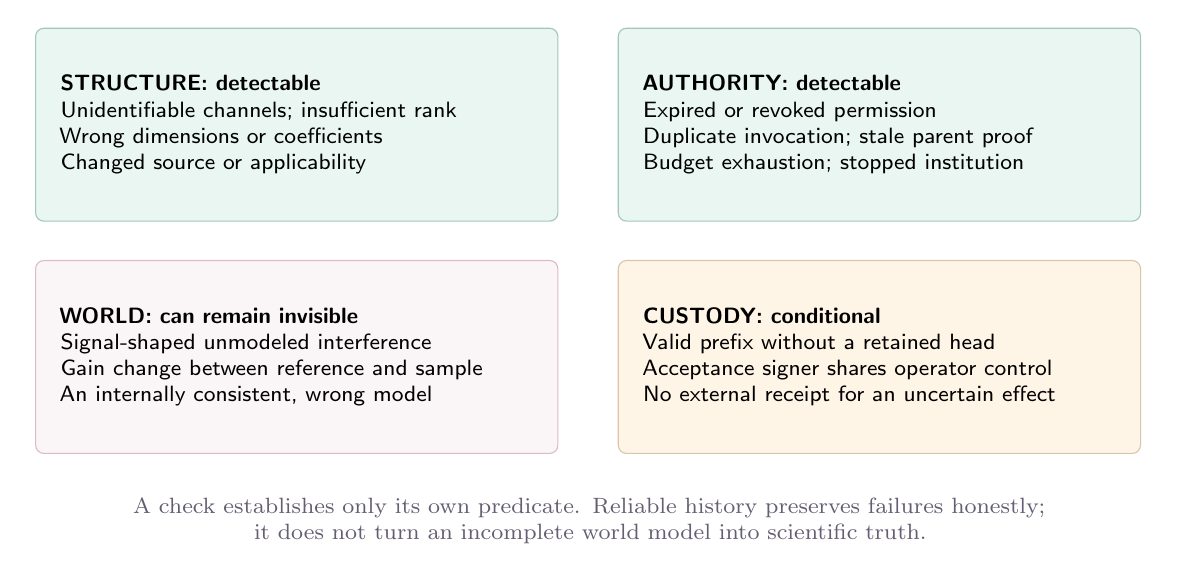
\begin{tikzpicture}[font=\sffamily\footnotesize,>=Stealth,
 box/.style={rounded corners=3pt,align=left,text width=6cm,inner sep=9pt,minimum height=2.45cm,anchor=north}]
\node[box,draw=Teal!40,fill=Mint] (a) at (0,0) {\textbf{STRUCTURE: detectable}\\Unidentifiable channels; insufficient rank\\Wrong dimensions or coefficients\\Changed source or applicability};
\node[box,draw=Teal!40,fill=Mint] (b) at (7.4,0) {\textbf{AUTHORITY: detectable}\\Expired or revoked permission\\Duplicate invocation; stale parent proof\\Budget exhaustion; stopped institution};
\node[box,draw=Rose!35,fill=Rose!5] (c) at (0,-2.95) {\textbf{WORLD: can remain invisible}\\Signal-shaped unmodeled interference\\Gain change between reference and sample\\An internally consistent, wrong model};
\node[box,draw=Amber!35,fill=Sand] (d) at (7.4,-2.95) {\textbf{CUSTODY: conditional}\\Valid prefix without a retained head\\Acceptance signer shares operator control\\No external receipt for an uncertain effect};
\node[text width=14cm,align=center,font=\footnotesize,text=Muted,anchor=north] at (3.7,-5.85) {A check establishes only its own predicate. Reliable history preserves failures honestly;\\it does not turn an incomplete world model into scientific truth.};
\end{tikzpicture}

% END input
}
\caption{An honest failure map. The companion exercises representative cases in each region. Green regions mean an observed applicable check, not exhaustive security coverage; the other regions mark assumptions the local demonstration cannot remove.}
\label{fig:failure-map}
\end{figure}

For real instrumentation, a next study would need an implemented modulator with independently selectable channel responses, detector characterization, noise and gain-drift measurements, independent references and a controlled comparison of acquisition time and hardware cost. Neither the binary response grammar nor polynomial cancellation proves that such hardware meets the model. The next useful artifact could be a physical validation protocol or a negative feasibility result, rather than a grander software lineage.

\subsection{Limits of the experiment}

The family is deliberately small and specified. Construction enumerates a supplied finite grammar using rational arithmetic; it is not autonomous discovery of photometry or a learned agent inventing an unrestricted new scientific technique. The held-out bank varies numerical conditions within the declared family. The scalar-to-dual and higher-order nuisance changes are meaningful output/model changes, but they are not evidence of transfer to arbitrary scientific domains.

The experiment uses a local process environment, public test signatures and one research controller. It does not test adversarial organizations, confidential data custody, independent human adjudication or malicious imported code. The runner's bounded tools are trusted local application code. STOP and expiry checks occur at defined execution boundaries; they do not preempt arbitrary running native code in real time.

Human authoring, integration and review effort was not measured prospectively. The engineering budget is comparable in available tools and shared infrastructure, not a measured equal labor allocation. Numerical work counts and descriptive host timing cannot establish a complete total-cost-of-ownership advantage. The local conventional baseline is scoped to the nominal workload and does not claim all the released runtime's governance or recovery features. Its observed faster timing must be interpreted within that narrower feature set.

No observed customer demand, financial return, real settlement, physical detector advantage or production fleet throughput is reported. The four-repository delivery restrictions are operational boundaries, not unresolved experimental results silently converted into success. This publication can be complete as a reproducible local study while those independent product decisions remain held.

\subsection{What would falsify the useful claim?}

The central claim would weaken if the constructed artifact failed exact independent replay, if a hidden model assumption explained away its quality, if the recipient could not interpret its applicability, or if compatibility and qualification consistently cost more than competent direct construction. A physical test that violates the assumed gain stability would invalidate the corresponding scientific bound. A demonstrated rollback of the journal without checkpoint detection would defeat the stated custody assumption. A claim of superior coverage would already be false for the frozen budget at which all four methods qualified every mission.

These are useful outcomes because the standard is retained productive capability under constraints, not uninterrupted narrative progress. A successor that cannot earn its current obligations should remain a proposal.

\begin{insight}[title={The contribution in one sentence}]
A completed mission can preserve the means of future work when its artifacts carry usable semantics and provenance, the successor constructs what changed, and current proof and authority are earned again---with the cost and the possibility of failure kept visible.
\end{insight}

% END input


% BEGIN sections/reproduction.tex
\section{Reproduction and the evidence docket}
\label{sec:reproduction}

The publication package contains the compiled PDF, complete LaTeX source, bibliography, editable vector figures, the research companion, original frozen protocols, raw observations, candidate failures, intervention disclosures, source audits and file hashes. Earlier source papers and development checkpoints are separate from the final experiment. A reproducible result is the specified computation and evidence, not a claim that future timestamps, signatures bound to those timestamps or machine timings will be byte-identical.

\subsection{Open the working demonstration}

The verified runtime environment is CPython 3.12.14 on Linux x86\_64. Scientific numerical code uses only the Python standard library. The released runtime closure additionally uses the exact dependencies listed in \path{companion/requirements.txt}; the complete pinned set includes Pydantic 2.14.1 and Cryptography 50.0.2. From the extracted package root:

\begin{quote}\small
\begin{verbatim}
python3 -m venv .venv
.venv/bin/python -m pip install -r companion/requirements.txt
.venv/bin/python companion/serve.py
\end{verbatim}
\end{quote}

Open the printed loopback address in a browser. The local interface offers the nominal journey, interrupted recovery and impossible successor. Each run creates a new evidence directory and exports a downloadable JSON evidence archive. The server accepts only these fixed scenarios, binds to the local computer and makes no external request. The separately provided standalone HTML is an interactive viewer of the recorded runs, clearly labelled as replay; fresh execution uses the local companion.

Setup may download pinned Python dependencies once. No model-provider credential or paid service is required. Full Alpha installation, ordinary private-key initialization and cross-repository installed-package acceptance are not part of these commands. Other interpreter/platform combinations may work but are not newly qualified by this study.

\subsection{Reproduce the science and inspect actual runtime evidence}

From the package root, the numerical study can be rerun without third-party libraries:

\begin{quote}\small
\begin{verbatim}
python3 companion/experiment/reproduce.py --output runs/science
\end{verbatim}
\end{quote}

The scientific verification record retains eighteen passing tests and a second execution of all 768 method--mission observations. Eleven comparison targets match exactly after excluding timing/environment fields, including the timing-free scientific digest. The original main results remain unchanged. The claim is exact reproduction of this finite generator and implementation, not a statistical guarantee about an unobserved world.

To execute and audit a new source-bound runtime journey:

\begin{quote}\small
\begin{verbatim}
.venv/bin/python companion/integration/run_integration.py \
  --output runs/nominal --scenario nominal
.venv/bin/python companion/integration/verify_evidence.py \
  runs/nominal
\end{verbatim}
\end{quote}

Use a fresh output directory. Substitute \code{crash} or \code{negative\_transfer} for the other scenarios. The two control runners, independent fixture audit and load-reproduction commands are documented in the component READMEs. The load study takes longer and should be run without competing local experiments if comparative timing matters. Its raw original timings remain authoritative for the reported table.

Verifying archived signatures and event heads establishes historical integrity relative to the public fixtures. It does not make an expired historical grant current. A new execution creates a new local fixture history and separately scoped current records; it does not revise the original experiment into a fresh approval.

\subsection{Rebuild the paper and verify the package}

The complete top-level \path{SUCCESSOR_Omega_Harness.tex} embeds the document sections, figure bodies and resolved bibliography. It compiles without shell escape, network access, hidden project files or external figures. With the recorded TeX Live packages, two \code{pdflatex} passes rebuild the PDF. The modular source under \path{paper/} remains editable and includes \path{references.bib}, figure sources and reproducible build scripts.

\path{MANIFEST.json} and \path{SHA256SUMS} bind the included payload files. \path{verify_manifest.py} checks their bytes without executing the scientific code. The reproduction record distinguishes exact scientific equality, runtime semantic verification, PDF rebuild identity and visual QA. It does not pretend that hardware timings should reproduce exactly. Every final PDF page is rendered and visually inspected, and the paper's numeric claims are checked against retained JSON rather than manually reconstructed results.

\begin{table}[htbp]
\centering\small
\begin{tabularx}{\linewidth}{P{.16\linewidth}Y P{.37\linewidth}}
\toprule
\textbf{Claim ID} & \textbf{Material claim} & \textbf{Supporting artifact}\\
\midrule
C01 & Exact scalar and joint cancellation, reconstruction and error bounds. & Scientific source, tests, capability JSONs; independent runtime auditor.\\
C02 & All four methods qualify 192/192 under the frozen budget; conventional tie and expert win. & \path{companion/experiment/results/summary.json}, raw results and campaign ledger.\\
C03 & Parent recipe consumed; first transition costs 49 additional operations. & Ancestor/successor demo contexts and scientific results note.\\
C04 & Two internally accepted scientific failures. & \path{companion/experiment/results/failure_map.json}.\\
C05 & Actual local dispatcher journey and preserved interruption/refusal. & Three final integration evidence directories, events and auditor reports.\\
C06 & Expiry, STOP, replay, custody and semantic limits. & Original 13-case controls and separately frozen two-case boundary controls.\\
C07 & Conventional nominal loop wins load overhead comparison. & Frozen benchmark protocol, all eighteen batch records and summary.\\
C08 & Current repository/contract functions and integration limits. & Source snapshots, source hashes and retained public coordination records.\\
C09 & Reproduction, complete source and inspected PDF. & Scientific verification record and package reproduction/visual-QA docket.\\
\bottomrule
\end{tabularx}
\caption{Reader's entry points into the machine-readable evidence docket. The detailed docket supplies exact paths, predicates and limitations for each claim; unknown or unrun connections are explicit.}
\label{tab:docket}
\end{table}

\subsection{Publication handoff}

The proposed paper ID is \code{successor-omega-harness-photometer-v1}. The handoff supplies exact PDF/TeX/archive identities, bilingual catalogue text and isolated source paths for the existing publication owner. Shared catalogue generation, required review, merge and served-byte verification remain that owner's process. The package does not replace any earlier paper, take ownership of the release lanes, or claim that an attachment is a published website.

% END input

\FloatBarrier
\begin{thebibliography}{25}
\providecommand{\natexlab}[1]{#1}
\providecommand{\url}[1]{\texttt{#1}}
\expandafter\ifx\csname urlstyle\endcsname\relax
  \providecommand{\doi}[1]{doi: #1}\else
  \providecommand{\doi}{doi: \begingroup \urlstyle{rm}\Url}\fi

\bibitem[Boucher(2026{\natexlab{a}})]{outdesign}
Vincent Boucher.
\newblock {Out-Design}: Creating the freedom to transform.
\newblock MONTREAL.AI revised research manuscript, October 2026{\natexlab{a}}.
\newblock URL
  \url{https://github.com/MontrealAI/AGI-Alpha-Agent-v0/blob/031bdb5d055c8bad896daa076baea2b5e17b242c/docs/Out_Design.pdf}.
\newblock 21 October 2026. Public filename Out\_Design.pdf; source-pinned at
  commit 031bdb5d055c8bad896daa076baea2b5e17b242c.

\bibitem[Boucher(2026{\natexlab{b}})]{outevolve}
Vincent Boucher.
\newblock {Out-Evolve}: Building the means of discovery and production.
\newblock MONTREAL.AI revised research manuscript, October 2026{\natexlab{b}}.
\newblock URL
  \url{https://github.com/MontrealAI/AGI-Alpha-Agent-v0/blob/031bdb5d055c8bad896daa076baea2b5e17b242c/docs/Out_Evolve.pdf}.
\newblock 20 October 2026. Canonical public edition; source-pinned at commit
  031bdb5d055c8bad896daa076baea2b5e17b242c.

\bibitem[Boucher(2026{\natexlab{c}})]{outexecute}
Vincent Boucher.
\newblock {Out-Execute}: Constructing the conditions of completion---from
  repeated work to reusable means of execution.
\newblock MONTREAL.AI revised research manuscript, October 2026{\natexlab{c}}.
\newblock URL
  \url{https://github.com/MontrealAI/AGI-Alpha-Agent-v0/blob/031bdb5d055c8bad896daa076baea2b5e17b242c/docs/Out_Execute.pdf}.
\newblock 21 October 2026. Public filename Out\_Execute.pdf; source-pinned at
  commit 031bdb5d055c8bad896daa076baea2b5e17b242c.

\bibitem[Boucher(2026{\natexlab{d}})]{outlearn}
Vincent Boucher.
\newblock {Out-Learn}: Change what you need to know---constructed experiments
  and sharp calibration guarantees for reusable learning.
\newblock MONTREAL.AI revised research manuscript, October 2026{\natexlab{d}}.
\newblock URL
  \url{https://github.com/MontrealAI/AGI-Alpha-Agent-v0/blob/031bdb5d055c8bad896daa076baea2b5e17b242c/docs/Out_Learn.pdf}.
\newblock 21 October 2026. Public filename Out\_Learn.pdf; source-pinned at
  commit 031bdb5d055c8bad896daa076baea2b5e17b242c.

\bibitem[Boucher(2026{\natexlab{e}})]{outstrategise}
Vincent Boucher.
\newblock {Out-Strategise}: Transformational intelligence for constructing the
  conditions of success.
\newblock MONTREAL.AI research manuscript, October 2026{\natexlab{e}}.
\newblock URL
  \url{https://github.com/MontrealAI/AGI-Alpha-Agent-v0/blob/031bdb5d055c8bad896daa076baea2b5e17b242c/docs/Out_Strategise.pdf}.
\newblock 20 October 2026. Source-pinned at commit
  031bdb5d055c8bad896daa076baea2b5e17b242c.

\bibitem[Boucher(2026{\natexlab{f}})]{outthink}
Vincent Boucher.
\newblock {Out-Think}: Transformational intelligence for inventing the space of
  reasoning.
\newblock MONTREAL.AI research manuscript, October 2026{\natexlab{f}}.
\newblock URL
  \url{https://github.com/MontrealAI/AGI-Alpha-Agent-v0/blob/031bdb5d055c8bad896daa076baea2b5e17b242c/docs/Out_Think.pdf}.
\newblock 21 October 2026. Source-pinned at commit
  031bdb5d055c8bad896daa076baea2b5e17b242c.

\bibitem[Boucher(2026{\natexlab{g}})]{ti}
Vincent Boucher.
\newblock Transformational intelligence: Learning to change the game.
\newblock MONTREAL.AI research manuscript, October 2026{\natexlab{g}}.
\newblock URL
  \url{https://github.com/MontrealAI/AGI-Alpha-Agent-v0/blob/031bdb5d055c8bad896daa076baea2b5e17b242c/docs/Transformational_Intelligence.pdf}.
\newblock Source-pinned at AGI-Alpha-Agent-v0 commit
  031bdb5d055c8bad896daa076baea2b5e17b242c.

\bibitem[Doiron(1993)]{doiron}
Ted Doiron.
\newblock Drift eliminating designs for non-simultaneous comparison
  calibrations.
\newblock \emph{Journal of Research of the National Institute of Standards and
  Technology}, 98\penalty0 (2):\penalty0 217--224, 1993.
\newblock \doi{10.6028/jres.098.016}.
\newblock URL \url{https://doi.org/10.6028/jres.098.016}.

\bibitem[Featonby()]{awsidempotency}
Malcolm Featonby.
\newblock Making retries safe with idempotent {APIs}.
\newblock Amazon Builders' Library.
\newblock URL
  \url{https://aws.amazon.com/builders-library/making-retries-safe-with-idempotent-APIs/}.
\newblock Accessed 24 October 2026.

\bibitem[Josefsson and Liusvaara(2017)]{rfc8032}
Simon Josefsson and Ilari Liusvaara.
\newblock Edwards-curve digital signature algorithm ({EdDSA}).
\newblock RFC 8032, January 2017.
\newblock URL \url{https://www.rfc-editor.org/rfc/rfc8032}.
\newblock Published test vectors used as deliberately public local fixtures,
  not production credentials.

\bibitem[Lee et~al.(2015)Lee, Park, Kejriwal, Matsushita, and
  Ousterhout]{lee_rifl2015}
Collin Lee, Seo~Jin Park, Ankita Kejriwal, Satoshi Matsushita, and John
  Ousterhout.
\newblock Implementing linearizability at large scale and low latency.
\newblock In \emph{Proceedings of the 25th ACM Symposium on Operating Systems
  Principles}, pages 71--86, 2015.
\newblock \doi{10.1145/2815400.2815416}.
\newblock URL \url{https://web.stanford.edu/~ouster/cgi-bin/papers/rifl.pdf}.

\bibitem[McConnell et~al.(2011)McConnell, Mehlhorn, N{\"a}her, and
  Schweitzer]{mcconnell_certifying2011}
Ross~M. McConnell, Kurt Mehlhorn, Stefan N{\"a}her, and Pascal Schweitzer.
\newblock Certifying algorithms.
\newblock \emph{Computer Science Review}, 5\penalty0 (2):\penalty0 119--161,
  2011.
\newblock \doi{10.1016/j.cosrev.2010.09.009}.
\newblock URL \url{https://www.cs.colostate.edu/~rmm/cert11.pdf}.

\bibitem[Mokhov et~al.(2018)Mokhov, Mitchell, and Peyton~Jones]{buildsystems}
Andrey Mokhov, Neil Mitchell, and Simon Peyton~Jones.
\newblock Build systems {\`a} la carte.
\newblock \emph{Proceedings of the ACM on Programming Languages}, 2\penalty0
  (ICFP):\penalty0 79:1--79:29, 2018.
\newblock \doi{10.1145/3236774}.
\newblock URL
  \url{https://www.microsoft.com/en-us/research/wp-content/uploads/2018/03/build-systems.pdf}.

\bibitem[{MONTREAL.AI}(2026{\natexlab{a}})]{alpha_source}
{MONTREAL.AI}.
\newblock {AGI ALPHA Agent}: Released runtime and ascension contract source,
  2026{\natexlab{a}}.
\newblock URL
  \url{https://github.com/MontrealAI/AGI-Alpha-Agent-v0/tree/031bdb5d055c8bad896daa076baea2b5e17b242c}.
\newblock Commit 031bdb5d055c8bad896daa076baea2b5e17b242c. Accessed 24 October
  2026.

\bibitem[{MONTREAL.AI}(2026{\natexlab{b}})]{coordination}
{MONTREAL.AI}.
\newblock {SUCCESSOR Omega}: Public integration coordination, issue 4850,
  2026{\natexlab{b}}.
\newblock URL
  \url{https://github.com/MontrealAI/AGI-Alpha-Agent-v0/issues/4850}.
\newblock Current ownership and restriction records accessed 24 October 2026;
  retained snapshot in source audit.

\bibitem[{MONTREAL.AI}(2026{\natexlab{c}})]{fleet_source}
{MONTREAL.AI}.
\newblock {AGI Fleet Linux}: Runtime and successor interface source,
  2026{\natexlab{c}}.
\newblock URL
  \url{https://github.com/MontrealAI/AGI-Fleet-Linux/tree/45759fb096faf8988f58ae5ea71248d0f35a97c7}.
\newblock Main 45759fb096faf8988f58ae5ea71248d0f35a97c7. Current integration
  candidate remains separately held.

\bibitem[{MONTREAL.AI}(2026{\natexlab{d}})]{jobs_source}
{MONTREAL.AI}.
\newblock {AGI Jobs v0}: Current source and discovery admission interface,
  2026{\natexlab{d}}.
\newblock URL
  \url{https://github.com/MontrealAI/AGIJobsv0/tree/9983478d42c32fe399f28dd9b0e0173f904b8a11}.
\newblock Main 9983478d42c32fe399f28dd9b0e0173f904b8a11; release rc.20 source
  f7c00e668fe31ce1ea907f0006b6c14dc9db5e01.

\bibitem[{MONTREAL.AI}(2026{\natexlab{e}})]{manager_source}
{MONTREAL.AI}.
\newblock {AGI Job Manager}: {USDC} route and source, 2026{\natexlab{e}}.
\newblock URL
  \url{https://github.com/MontrealAI/AGIJobManager/tree/c5958eae872458c2f3cac48fea0b4bbfadc6ac6c}.
\newblock Commit c5958eae872458c2f3cac48fea0b4bbfadc6ac6c; release v1.20.1.

\bibitem[{MONTREAL.AI}(2026{\natexlab{f}})]{priorharness}
{MONTREAL.AI}.
\newblock Transformational autonomous enterprises: Mission-relative
  revalidation for capability inheritance across four execution systems,
  2026{\natexlab{f}}.
\newblock URL
  \url{https://github.com/MontrealAI/AGI-Alpha-Agent-v0/blob/031bdb5d055c8bad896daa076baea2b5e17b242c/docs/papers/transformational-autonomous-enterprises-v1.pdf}.
\newblock Writer 4 research edition, 23 October. Prior original; not rerun by
  this study.

\bibitem[Moreau and Missier(2013)]{prov}
Luc Moreau and Paolo Missier.
\newblock {PROV-DM}: The {PROV} data model.
\newblock W3c recommendation, World Wide Web Consortium, April 2013.
\newblock URL \url{https://www.w3.org/TR/prov-dm/}.
\newblock Editors. 30 April 2013.

\bibitem[Necula(1997)]{pcc}
George~C. Necula.
\newblock Proof-carrying code.
\newblock In \emph{Proceedings of the 24th ACM SIGPLAN-SIGACT Symposium on
  Principles of Programming Languages}, pages 106--119, 1997.
\newblock \doi{10.1145/263699.263712}.
\newblock URL \url{https://people.eecs.berkeley.edu/~necula/papers.html}.

\bibitem[{SQLite}()]{sqlite_wal}
{SQLite}.
\newblock Write-ahead logging.
\newblock SQLite documentation.
\newblock URL \url{https://www.sqlite.org/wal.html}.
\newblock Accessed 24 October 2026.

\bibitem[{SQLite}(2026)]{sqlite}
{SQLite}.
\newblock Transaction.
\newblock SQLite documentation, 2026.
\newblock URL \url{https://www.sqlite.org/lang_transaction.html}.
\newblock Page updated 18 February 2026; accessed 24 October 2026.

\bibitem[Swanson and Schlamminger(2010)]{swanson}
H.~Erik Swanson and Stephan Schlamminger.
\newblock Removal of zero-point drift from {AB} data and the statistical cost.
\newblock \emph{Measurement Science and Technology}, 21\penalty0 (11):\penalty0
  115104, 2010.
\newblock \doi{10.1088/0957-0233/21/11/115104}.
\newblock URL \url{https://arxiv.org/abs/1009.1894}.

\bibitem[{Temporal Technologies}(2026)]{temporal}
{Temporal Technologies}.
\newblock Activity definition.
\newblock Temporal documentation, 2026.
\newblock URL \url{https://docs.temporal.io/activity-definition}.
\newblock Accessed 24 October 2026.

\end{thebibliography}

\clearpage
\appendix

% BEGIN sections/appendix.tex
\section{Exact identities and interpretation rules}

\subsection{Repository pins}

\begin{description}[style=nextline,leftmargin=1em,font=\sffamily\bfseries\small]
\item[Alpha / released-source dependency closure]
\path{031bdb5d055c8bad896daa076baea2b5e17b242c}
\item[Jobs / audited main]
\path{9983478d42c32fe399f28dd9b0e0173f904b8a11}
\item[Jobs / rc.20 product source]
\path{f7c00e668fe31ce1ea907f0006b6c14dc9db5e01}
\item[Manager / v1.20.1]
\path{c5958eae872458c2f3cac48fea0b4bbfadc6ac6c}
\item[Fleet / audited main]
\path{45759fb096faf8988f58ae5ea71248d0f35a97c7}
\end{description}

The Alpha annotated release tag object was independently resolved and peeled to the same commit. The audit observes the public v1.41.0 asset set without repeating its previous owner-controlled acceptance. Exact bytes of the eleven vendored runtime files are listed in \path{companion/integration/VENDOR_MANIFEST.json} and compared with source in the fixture audit.

\subsection{Frozen research identities}

\begin{description}[style=nextline,leftmargin=1em,font=\sffamily\bfseries\small]
\item[Primary protocol SHA-256]
\path{cb3a71483ade02deb1c835b8a5358dc728d87ed29d7df48812d97940e586f263}
\item[Scientific implementation SHA-256]
\path{ea7d3a4cc01a3733c8983899f95ed8ae93a5ca79a8efc2ae7a8e56894dc78c2b}
\item[Timing-free primary scientific digest]
\path{da9d53f64df6bd369f166a42483ea60ea05c0c8c891ddc73e0d10304b07112a3}
\item[Load protocol SHA-256]
\path{caa3ebf06be4f33c2ed02b5326381f711c7635692bd1f0e932d5818b59607689}
\item[Integration source-manifest SHA-256]
\path{aca0b11952b259dddf289942b645cb82b9a48b7c789e135c7cc496d3d7c61eab}
\end{description}

The pre-main clarification preserves the original protocol bytes and adds the actual parent-recipe use, complete bounded-noise formula and cost-counting scope. It changes no seed, candidate library, quality threshold, budget or stopping rule. Implementation review occurred before main evaluation. Later deterministic candidate enumeration is labelled as a supplementary audit; it does not replace the main campaign.

\section{Candidate failures and stage evidence}

The finite candidate audit records one admitted scalar program, all forty-five quadratic joint candidates meeting quality, twenty-six of forty-five cubic joint candidates meeting quality, and no admissible quartic joint candidate within six readings. The cubic failures include six singular designs and thirteen that exceed the risk threshold. Failed proposals remain in the evidence package. Selecting a successful candidate does not erase the work spent evaluating the others.

\begin{table}[htbp]
\centering\small
\begin{tabularx}{\linewidth}{P{.19\linewidth}Y Y}
\toprule
\textbf{Stage} & \textbf{Inspectable artifact} & \textbf{Contribution and limit}\\
\midrule
Identify & Rank of unmodulated signal/nuisance design and mission specification. & Exposes confounding; does not infer a true physical world model.\\
Out-Learn & Source-bound symbolic recipe and its evaluated basis. & Actual reusable representation; the first transition adds verification cost.\\
Out-Think & Dimension feasibility and explicit identity/error obligations. & Early explanation of infeasibility; later inverse checks are also protective.\\
Out-Design & Response matrix, exact decoder, candidate dispositions. & Constructs the new interface; supplied finite grammar limits novelty.\\
Out-Strategise & Proposed acquisitions versus cap; execute/stop decision. & Stops a costly inadmissible plan; not a learned economic optimizer.\\
Out-Execute & Raw readings, gain/signal intervals and fresh receipt. & Qualified synthetic measurement; gain/interference assumptions can fail invisibly.\\
Out-Evolve & Accepted-parent record, recipe provenance and new requirement. & Retains usable history; neither current child proof nor production permission transfers.\\
\bottomrule
\end{tabularx}
\caption{The executed stage map is deliberately narrower than the ambitions of each source paper. Per-stage counters, artifacts and receipts appear in the exported contexts.}
\end{table}

\section{Threats to validity and future qualification}

\textbf{Model validity.} The simulator enforces the declared noise and drift family in the main campaigns. Physical errors may exceed the declared componentwise bound, gain may change, and background may leave the declared polynomial span; correlation within the bound does not invalidate the deterministic guarantee. Measurement timing and independently selectable responses are assumed. The two missed controls demonstrate that an exact internal check cannot certify those assumptions.

\textbf{Selection and comparison.} The task grammar and response library are researcher-supplied. The main seed bank is held out from construction, but it is not an adversarially selected external task distribution. The expert-coded constructor is a competent program, not measured human expertise. Equal tools and callbacks do not establish equal human development budgets. The direct durable loop is explicitly narrower than the full lifecycle implementation.

\textbf{Implementation and custody.} Exact rational tests are not formal verification of Python, the runtime, SQLite, the operating system or cryptographic libraries. Filesystem durability assumes the documented host/storage behavior \cite{sqlite,sqlite_wal}. Public signature fixtures provide no production identity. Journal-prefix detection needs a retained checkpoint outside an attacker's permitted rollback set.

\textbf{Reproduction and time.} Numerical outcomes reproduce with the specified interpreter and generator. Journal timestamps and new authorizations change on rerun. Load timing is descriptive on one shared machine; no confidence interval for all future workloads is implied. Package verification checks delivered bytes, while rerunning science or runtime behavior is a different claim.

\textbf{Deployment and economics.} The paper does not supply an installed four-repository journey, commissioned customer work, paid settlement or complete labor cost. Any future scientific hardware, service route, contract interaction or production authorization needs its own exact-source and current-world qualification. Existing held operations remain held until their proper owners resolve them.

\section{Research and authorship disclosure}

The study and manuscript were prepared for MONTREAL.AI with AI-assisted research, implementation and review. Separate review roles within the same production process are disclosed as such; they are not represented as independent institutions or peer review. No human-participant experiment was conducted. There were no demo-initiated currency transfers. Research-model usage, host allocation, electricity and human authoring/review costs are unknown. Original source papers, early development artifacts, failed proposals and later corrections are retained with their own identities.

% END input

\end{document}
